% --------------------------------------------------------------------

\chapter{The Galaxy}
\def\chpname{galaxy}\label{chp:\chpname}

Chapter editors:
\credit{willclarkson},
\credit{akvivas}.

Contributing authors:
\credit{bethwillman},
\credit{dnidever},
\credit{ivezic},
\credit{ctslater},
\credit{pmmcgehee},
\credit{cbritt4},
\credit{dgmonet},
\credit{caprastro},
{\it Dana Casetti, John Gizis, Michael Liu and others to follow}


% --------------------------------------------------------------------

\section{Introduction}
\def\secname{MW_Intro}\label{sec:\secname}

LSST's large survey grasp will yield significant contributions to
essentially all areas of Galactic astronomy. Science cases for Milky
Way astronomy with LSST cover lengthscales from a few pc (such as
sensitive surveys of low-mass objects in the Solar Neighborhood), up
to many tens of kpc (such as sensitive surveys for low-mass satellite
galaxies of the Milky Way and their post-disruption remnant streams,
and beyond this, investigations of resolved stellar populations in the
Local Volume). 

Because the diversity of science cases in the Milky Way is so vast, we
make no attempt to be comprehensive. Much more detail about most of
the LSST science cases, and specific science questions to be answered,
can be found in the LSST Science Book (particularly chapters 6 and 7)
and Ivezic et al. (2008 arXiv 0805.2366, in particular Sections 2.1.4
and 4.4 of that document).\footnote{\new{Since several of the science cases
for populations in the Galactic Disk do not appear to have been developed
elsewhere, however, Section~\ref{sec:MW_Disk} does present motivating details
for those science cases.}} In this chapter we present a few
representative science cases that illustrate trade-offs between
observing strategies, for programs at low galactic latitudes as well
as away from the disk, and for programs requiring sufficient cadence
for variability as well as deep integrated imaging. 

As with the rest of this whitepaper, our intention is to provoke the
astronomical community to contribute to the optimization of LSST's
observing strategy. Readers who find that an important area of Milky
Way astronomy is under-served by the treatment here, are welcome to
contact the editors to get involved and contribute improvements. For
example, while inclusion of the inner Galactic plane in the
Wide-Fast-Deep survey would allow characterization of important
populations through variability (as will be shown quantitatively in
Section 4.3), such a dataset would also be of immense value in
disentangling and measuring structural parameters of major galactic
components (for example the tilt angle of the disk and the effects of
radial migration within it). We welcome further development of
quantitative figures of merit by which the appropriateness of LSST's observing
strategies can be assessed in terms of the science of interest to the
reader.

\subsection{Chapter terminology and structure}

In what follows, ``Metrics'' refer to diagnostic metrics of LSST's
technical performance, and are generally rather low-level (for
example, the formal proper motion precision, mapped with location
across the sky). Then, a ``figure of merit'' is a higher-level
quantity that illustrates LSST's utility for the science case of
interest (for example, the uncertainty and/or bias on an astrophysical
parameter of interest, such as the mass function of a certain stellar
population near the Sun).

To try to tame the diversity of science cases, we have picked
representative cases and grouped them within broad scientific areas,
devoting one Section of this chapter to each grouping of cases. Our
intention at this date is to provide a summary Table at the end of
each Section that will present the figure of merit for each science
case within that section (as columns) for each tested observing
strategy (as rows).

At present, science cases are grouped in the following way:
Section~\ref{sec:MW_Halo} assesses the degree to which structures in the Milky
Way's halo can be discriminated and mapped, using tracer populations
distinguished by variability and derived stellar parameters.
Section~\ref{sec:MW_Disk} assesses the impact of observing strategy on LSST's
ability to map some representative astrophysically important
populations that are found mostly or exclusively in the Plane
(including Dust in the ISM). Several observational challenges for LSST
find their sharpest expression in Milky Way science, including (but
not limited to) measurements of stellar parallax, absolute astrometry,
and proper motions (including the tie-in to the reference frame which
will be provided by the \textit{Gaia} mission). For this reason, specific
issues relating to precision astrometry are developed in
Section~\ref{sec:MW_Astrometry}.

\new{Section \ref{sec:MW_Future} presents descriptions of
  investigations that are needed to properly determine LSST's utility
  for Milky Way science, but which at this date (mid-April 2016) are
  as-yet relatively incompletely developed. Examples identified at
  this stage include the uses of LSST to set constraints on Galactic
  components (the structure of the Bulge, and constraints on radial
  migration in the mid-plane).}

\subsection{Summary tables for Figures of Merit}

\new{At-a-glance tables comparing Figures of Merit for the various science
cases, will be found in the appropriate summary tables:}
\begin{itemize}
  \item Mapping the Milky Way Halo: Table \ref{tab_SummaryMWHalo}
  \item Mapping the Milky Way Disk: Table \ref{tab_SummaryMWDisk}
  \item Astrometry with LSST: Table \ref{tab_SummaryMWAstrometry}
  \item The Milky Way Bulge: content needed
  \item Mapping the Local Volume with Resolved Stars: content needed.
\end{itemize}

\subsection{Needed input}

Many of the diagnostic Metrics are (as of February 2016) relatively
well-developed. What is needed at this stage is the implementation of
the figures of merit that depend on these Metrics. In some Sections we
have sketched out such figures of merit, in others the development of
a useful (and practical) figure of merit is still a topic of active
development. 

We welcome assistance from the reader in the development of the
figures of merit for all sections. 

% ====================================================================
%+
% SECTION:
%    section-name.tex  % eg lenstimedelays.tex
%
% CHAPTER:
%    chapter.tex  % eg cosmology.tex
%
% ELEVATOR PITCH:
%    Explain in a few sentences what the relevant discovery or
%    measurement is going to be discussed, and what will be important
%    about it. This is for the browsing reader to get a quick feel
%    for what this section is about.
%
% COMMENTS:
%
%
% BUGS:
%
%
% AUTHORS:
%    Phil Marshall (@drphilmarshall)  - put your name and GitHub username here!
%-
% ====================================================================

\section{Mapping the Milky Way Halo}
\def\secname{MW_Halo}\label{sec:\secname} % For example, replace "keyword" with "lenstimedelays"

\noindent{\it Kathy Vivas, Colin Slater, David Nidever, Beth Willman}  % (Writing team)

The study of the Halo of the Milky Way is of the most importance not only to understand
the formation and early evolution of our own galaxy, but also to test 
test current models of hierarchical galaxy formation. 
LSST will provide an unprecedented combination of
area, depth, multi-band, multi-epoch information for pursuing detail studies
of the structure of this old Galactic component. We focus here in three
specific projects that can be pursued with LSST. We suggest metrics and figure of merits that can
be calculated in order to quantify the feasibility of the projects under different
observational strategies. We expect more projects will join later.

RR Lyrae stars have been known for several decades as excellent tracers
of the halo population. They are not only old stars ($>10$ Gyrs) but they are
also excellent standard candles that allow to build 3-dimensional maps. 
The halo of the Milky Way has been now surveyed in a very large extension up to 
$\sim 60-80$ kpc from the Galactic center \citep[][among others]{drake13a,drake13b,zinn14,torrealba15}. 
Beyond that, the halo is
mostly uncharted territory.
From these RR Lyrae surveys, we have learned that the halo is filled with substructures
which are usually interpreted as debris from destroyed satellite galaxies. The smooth 
component of the RR Lyrae distribution is well described
with a power-law of the mean number density of RR Lyrae stars as a function of
galactocentric distance, which gets steeper after $\sim 30$ kpc \citep{zinn14}. 
Thus, beyond $\sim 60$ kpc, few field RR Lyrae stars are expected. However, we presume that 
any RR Lyrae star beyond this distance may be part of either debris material or distant
satellite galaxies of low luminosity that have been escaped detection until now \citep{sesar14,baker15}. 
LCDM models predict debris as far as $0.5$~Mpc from the galactic center
This is the territory that will be explored by LSST.

Similarly, red giant stars can be used to trace the structure of the halo up to large
distances. They have the advantage 
of being bright and numerous stars.

Fainter than these two tracers, main sequence stars stand up as a tool for studying
the Halo. They are the most numerous type of stars available and statistical studies 
are possible. Using the technique of photometric metallicities \citep{ivezic08}, 
SDSS provided unprecedented maps of the metallicity distribution up to  $\sim 10$ 
kpc from the Galactic center, unveiling not only the mean metallicity distribution 
of the halo but also, sub-structures within the halo. This kind of works will be extended
to the outermost parts of the Galaxy with LSST data.


% --------------------------------------------------------------------

\subsection{Target measurements and discoveries}
\label{sec:\secname:MW_Halo_targets}

The three projects just described require the discovery and/or measurement of the following 
type of objects:

\begin{itemize}

\item RR Lyrae stars: These are bright horizontal-branch variable stars with
periods between 0.2 to 1.0 days and large amplitudes, particularly in the bluer 
bandpasses (g amplitudes $0.5 - 1.5$~mag). \citet{2012AJ....144....9O} made an intensive
search for RR Lyrae stars in simulated LSST data and reached to the conclusion 
that this type of stars can be recovered to distances $\sim 600$ kpc. A similar procedure
can now be performed using MAF and current cadence scenarios.
Chapter \ref{chp:variables} discusses the discovery metrics for variable stars 
including RR Lyrae stars. However, optimal recovery may involve more complex metrics
involving the simultaneous use of multi-band time series \citep{vanderplas15,vivas16}.
Besides the recovery of the variable stars, a particularly valuable measurement to track 
for studies in the halo is the infrared mean magnitudes z and y since they provide the 
most accurate way to obtain distances \citep{caceres08}. 

\item Main sequence stars: lacking any distinguishable variability, the
challenge in selecting a large and clean sample of main sequence stars comes
from tremendous number of small and nearly-unresolved galaxies present at
faint magnitudes. Precise star/galaxy separation is thus the limiting factor
on the useful depth of the main sequence sample. In addition to identifying
dwarfs, using dwarfs to map the metallicity distribution of the halo requires
precise u-band data, since it exhibits the strongest metallicity dependence of
the LSST filters.

\item Red Giants: due to their intrinsic luminosity red giants will be sample
a far deeper volume than main sequence stars at similar apparent magnitudes,
but they must first be identified and separated from the very numerous main
sequence stars present in the field. A gravity-sensitive photometric index can
be used for separating efficiently giants from dwarfs. The u magnitude
is an essential ingredient in this process and it is necessary to follow-up
the behavior of the u limiting magnitude under different observational
strategies. Figure~\ref{fig-MW-giants} shows the distance that can be reached 
by M giants of different metallicities assuming a limiting magnitude in the u band of
26.0. 

\end{itemize}

\begin{figure}
\begin{center}
  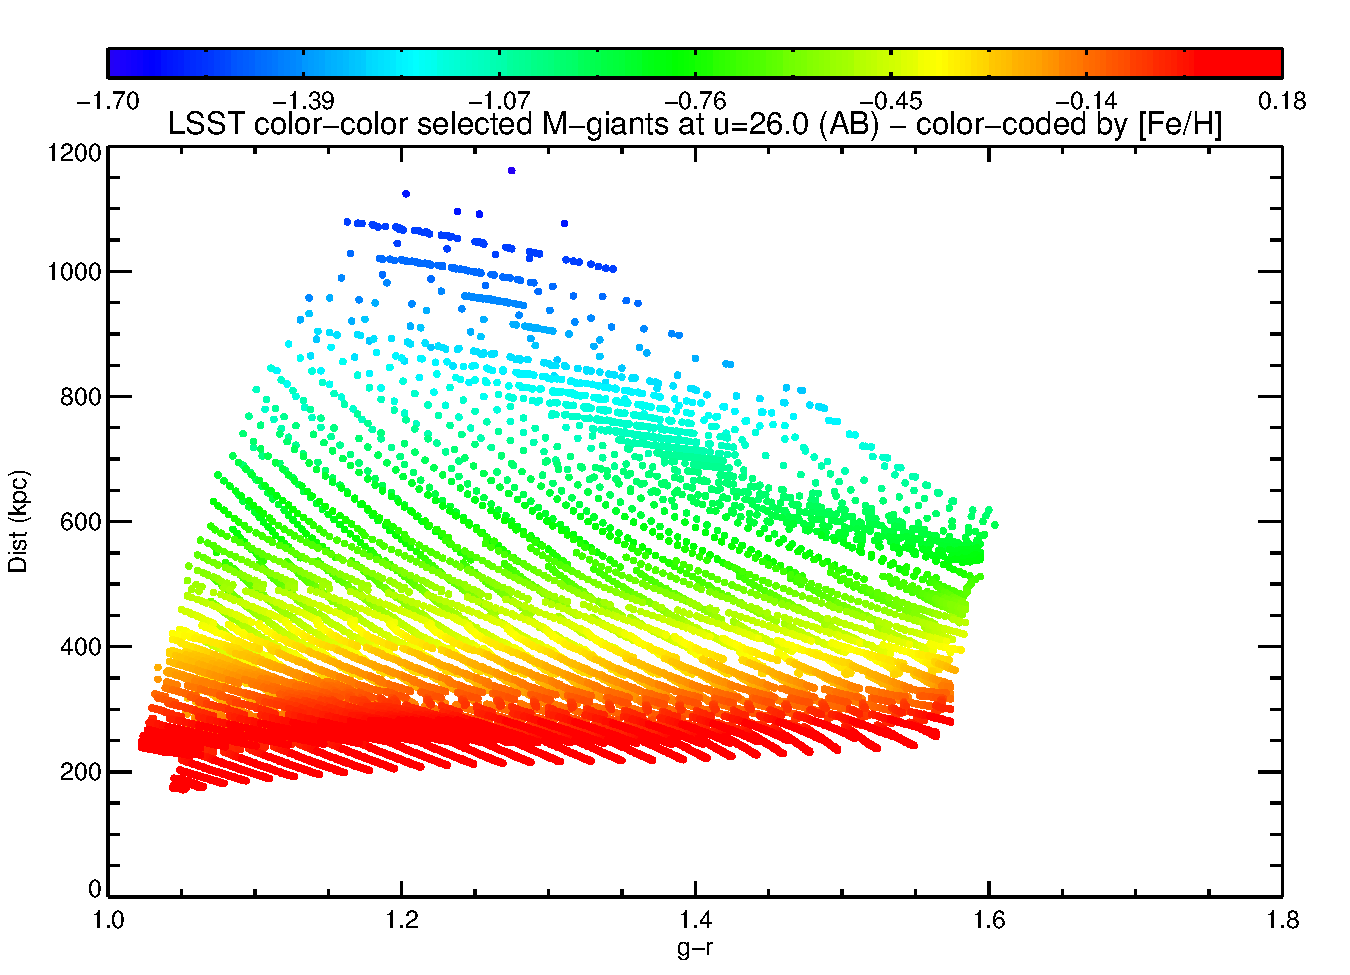
\includegraphics[scale=0.5]{./figs/milkyway/lsst_mgiants_grdist.pdf}
  \caption{Distance to which red giant stars can be identified in the galactic halo asuuming a limiting magnitude
  of u=26.0. The color code scales with the metallicity of the stars. More metal-poor stars can be 
  detected to farther distances. \label{fig-MW-giants}}
\end{center}
\end{figure}


% --------------------------------------------------------------------

\subsection{Metrics}
\label{sec:\secname:MW_Halo_metrics}

\textbf{Star-Galaxy Separation:} For main sequence stars, the useful depth of
the survey will likely not be the photometric detection limit but will instead
be set by the ability to differentiate stars from unresolved background
galaxies. Towards faint magnitudes the contamination by galaxies worsens
significantly for several reasons: the number of galaxies is rising
substantially, the angular size of galaxies is shrinking, and our ability to
distinguish stars from marginally resolved galaxies diminishes for faint
sources simply due to photon statistics. While the fundamental properties of
the contaminant sources is beyond our control, our ability to reject these
sources depends on survey parameters such as the distribution of seeing across
visits and the depth of these visits.

We are currently in the process of developing a metric that will estimate our
ability to separate stars and galaxies for any observation depth and seeing
conditions. This requires both an understanding of how images of a source are
measured and classified as either a star or galaxy, and how the population of
stars and galaxies vary in number and size (for galaxies) with depth. Our model
uses the distribution of galaxies in size and number, derived from HST COSMOS
observations, along with a fully Bayesian model decision formalism to compute
the expected completeness and contamination in star-galaxy separation.
Computationally for each position in the survey footprint we interpolate the
results from that work on a grid in seeing, galaxy size, and coadd depth, then
integrate over the distribution of galaxy sizes. This modeling process is
currently being verified against existing surveys, and will be incorporated into
the observing strategy study at a later date.

\textbf{Distance to the farthest RR Lyrae stars:} This metrics involves the ability to
recover an RR Lyrae star as a function of its distance. An RR Lyrae star may be
considered as recovered if its period and amplitude are within 10\% of their real values.
The distance is calculated using the mean magnitude of the recovered RR Lyrae stars 
(in the more IR photometrics bands) and the interstellar extinction (maps are available 
now in MAF).  Output of this metric is the distance at which certain percentage of RR 
Lyrae stars (eg. 80\%) can be recovered by LSST. It is expected that the results 
of this metric at low galactic latitudes will be largely dependent on the chosen observational 
strategy. 

A reasonable Figure of Merit for this sub-project is the volume of the halo within RR Lyrae stars 
can be recovered. Similarly, another Figure of Merit is the fraction of the Galactic thick disk's volume that can be 
traced by RR Lyrae stars.

\textbf{Distance to the farthest main sequence stars and giant stars:} Being non-variable objects
the metrics for these objects are somewhat simpler and requires the determination of the limiting
magnitude (in u band) for which galaxy/star separation is reliable to certain level. Then, a figure of
merit is the volume of the halo mapped with these tracers. 



% --------------------------------------------------------------------

\subsection{OpSim Analysis}
\label{sec:\secname:MW_Halo_analysis}

Table \ref{tab_SummaryMWHalo} summarizes the science Figures of Merit
for the Milky Way Halo science cases for LSST. OpSim analysis for this
Section will be summarized in that Table; at the present date (April
2016) placeholder rows are given for the FoM's. Input from the readers
is welcome!

%%% SUMMARY TABLE FOR THIS SUBSECTION

\begin{table}
  \begin{tabular}{l|p{6cm}|c|c|c|c|p{5cm}}
    FoM & Brief description & {\rotatebox{90}{\opsimdbref{db:baseCadence} }} & {\rotatebox{90}{\opsimdbref{db:opstwoPS} }} & {\rotatebox{90}{future run 1}} &  {\rotatebox{90}{future run 2}} & Notes \\
    \hline
    1.1. & \footnotesize{Survey volume to RR Lyraes}      & - & - & - & - & \footnotesize{Volume within which the distance to a template RR Lyrae star can be estimated to 10\% uncertainty.} \\
    1.2. & \footnotesize{Survey volume to Main Sequence tracers} & - & - & - & - & \footnotesize{(Including star-galaxy separation)} \\
    1.3. & \footnotesize{Survey volume to Red Giants} & - & - & - & - & - \\
%    2.1. & \footnotesize{Completeness of metallicity sub-structure recovery as a function of distance} & - & - & - & - & \footnotesize{Over all three tracer populations?} \\ 
%    3.1. & \footnotesize{Uncertainty and bias in age distribution parameterization of the main Halo population} & - & - & - & - & - \\
%    3.2. & \footnotesize{Uncertainty and bias in the population fraction identified correctly with each halo component} & - & - & - & - & \footnotesize{Some overlap with Halo astrometry FoM?} \\
\end{tabular}
\caption{Summary of figures-of-merit (FoMs) for the Galactic Halo science cases. The best value of each FoM is indicated in bold. Runs \opsimdbref{db:baseCadence} and \opsimdbref{db:opstwoPS} refer to the Baseline and PanSTARRS-like strategies, respectively. See Section \ref{sec:MW_Halo}.}
\label{tab_SummaryMWHalo}
\end{table}


% --------------------------------------------------------------------

%\subsection{Discussion}
%\label{sec:\secname:MW_Halo_discussion}

%Discussion: what risks have been identified? What suggestions could be
%made to improve this science project's figure of merit, and mitigate
%the identified risks?


% ====================================================================

\navigationbar

% ====================================================================
%+
% SECTION:
%    section-name.tex  % eg lenstimedelays.tex
%
% CHAPTER:
%    chapter.tex  % eg cosmology.tex
%
% ELEVATOR PITCH:
%    Explain in a few sentences what the relevant discovery or
%    measurement is going to be discussed, and what will be important
%    about it. This is for the browsing reader to get a quick feel
%    for what this section is about.
%
% COMMENTS:
%
%
% BUGS:
%
%
% AUTHORS:
%    Phil Marshall (@drphilmarshall)  - put your name and GitHub username here!
%-
% ====================================================================

\section{Mapping the Milky Way Disk}
\def\secname{MW_Disk}\label{sec:\secname} % For example, replace "keyword" with "lenstimedelays"

\noindent{\it Will Clarkson, Peregrine McGehee, Jay Strader, Chris Britt}  % (Writing team)

% This individual section will need to describe the particular
% discoveries and measurements that are being targeted in this section's
% science case. It will be helpful to think of a ``science case" as a
% ``science project" that the authors {\it actually plan to do}. Then,
% the sections can follow the tried and tested format of an observing
% proposal: a brief description of the investigation, with references,
% followed by a technical feasibility piece. This latter part will need
% to be quantified using the MAF framework, via a set of metrics that
% need to be computed for any given observing strategy to quantify its
% impact on the described science case. Ideally, these metrics would be
% combined in a well-motivated figure of merit. The section can conclude
% with a discussion of any risks that have been identified, and how
% these could be mitigated.

%A short preamble goes here. What's the context for this science
%project? Where does it fit in the big picture?

Many populations of great importance to Astronomy exist predominantly
in or near the Galactic Plane, and yet are sufficiently
sparsely-distributed (and/or faint enough) that LSST is likely to be
the only facility in the forseeable future that will be able to
identify a statistically meaningful sample. Some (such as the novae
that allow detailed study of the route to Type Ia Supernovae) offer
unique laboratories to study processes of fundamental importance to
astrophysics at all scales. Others (like intra-disk microlensing
events) offer the {\it only} probe of important populations. An
important collateral benefit of studies in the plane with an LSST-like
facility, is improved mapping of the distribution and observational
effects of the ISM (particularly dust), which is of importance to all
IR/Optical/UV observational studies.

% --------------------------------------------------------------------

\subsection{Target measurements and discoveries}
\label{sec:\secname:MW_Disk_targets}

%Describe the discoveries and measurements you want to make.

%Now, describe their response to the observing strategy. Qualitatively,
%how will the science project be affected by the observing schedule and
%conditions? In broad terms, how would we expect the observing strategy
%to be optimized for this science?

We have identified five science cases within the general area of Milky
Way Disk studies, that will have a diversity of dependencies on
observing strategy (e.g. slow intrinsic variability vs fast intrinsic
variability vs no variability). When the figures of merit have been
computed for these science cases, the results will be summarized in a Table in Section~\ref{sec:\secname:MW_Disk_discussion}.

\begin{itemize}
  \item 1. Quantifying the large quiescent compact binary population via variability;
  \item 2. New insights into the behavior of Novae and the route to Type Ia Superovae;
  \item 3. The next Galactic Supernova;
  \item 4. Measuring population parameters of planets outside the Snow Line with Microlensing;
  \item 5. A three-dimensional Dust map and improvements in the reddening law
\end{itemize}

Motivation and qualitative description of response to observing strategy:

{\bf 1. Probing quiescent compact binaries via variability:} Of the
millions of stellar-mass black holes formed through the collapse of
massive stars over the lifetime of the Milky Way, only $\sim 20$ have
been dynamically confirmed through spectroscopic measurements (e.g.,
Corral-Santana et al.~2015). Many questions central to modern
astrophysics can only be answered by enlarging this sample: which
stars produce neutron stars and which black holes; whether there is a
true gap in mass between neutron stars and black holes; whether
supernova explosions result in large black hole kicks. 

There is expected to be a large population of black hole binaries in quiescence
with low X-ray luminosities from $\sim 10^{30}$--$10^{33}$ erg/s.
Such systems can be identified as optical variables that show unique,
double-humped ellipsoidal variations of typical amplitude $\sim 0.2$
mag due to the tidal deformation of the secondary star, which can be a
giant or main sequence star. In some cases analysis of the light curve
alone can point to a high mass ratio between the components,
suggesting a black hole primary; in other cases the accretion disk
will make a large contribution to the optical light which results in
intrinsic, random, and fast variations in the light curve. The disk
contribution to optical light can change over time, and several years
of data is necessary to properly subtract the accretion disk
contribution in order to properly fit ellipsoidal veriations (Cantrell
et al. 2010). The brighter sources will be amenable to spectroscopy
with the current generation of 4-m to 10-m telescopes to dynamically
confirm new black holes; spectroscopy of all candidates should be
possible with the forthcoming generation of large telescopes. Thus,
LSST would trigger a rich variety of observational investigations of
the accretion/outflow process through studies of this large, dark
population.

While we have focused above on black hole binaries, we note that LSST
would be crucial for investigations of neutron star and white dwarf
binaries. For example, the total number of compact binaries 
is presently
poorly understood---Population models of neutron star X-ray binaries diverge by orders 
of magnitude, largely due to uncertainties in the common envelope phase of binary evolution (e.g. Pfahl et al, 2003; Kiel \& Hurley, 2006; van Haaften et al, 2015). This is
poorly constrained but has a large impact on, for example, LIGO event
rates. A simple test case of common envelope evolution is available in the number of dwarf novae (DNe) 
(accretion disk instability outbursts around white dwarfs), a population that does not suffer from
some of the complicating factors that neutron star and black hole binaries do (e.g. supernova kicks). 
Theoretical estimates routinely yield a significantly higher number of DNe than are observed in the solar
neighborhood. Understanding the true specific frequency of these
systems provides a key check on common envelope evolution.  LSST will detect dwarf novae, which last at least several days
with typical amplitudes of 4--6 mag,
out to kpc scales. This will allow a test of not only the number of
cataclysmic variables, but also of the 3D distribution within the
Galaxy and dependence on metallicity gradients (Britt et al. 2015).

{\it Response to observing strategy:} Since most black hole candidates
have been identified near the plane in the inner Milky Way (68\%, 92\%
within $5^{\circ}, 10^{\circ}$~of the Plane), this science case {\it
    requires} that LSST observe the plane with sufficient cadence to
  detect the $\sim$hundreds of quiescent black-hole binaries by virtue
  of their variability. The natural choice for a survey for
  low-luminosity black hole binaries would be to extend the
  Wide-Fast-Deep survey throughout the Plane in the direction of the
  inner Milky Way. The orbital period of these systems is short (typically $<1$ day), so that a rolling cadence
  for at least parts of the Plane should be considered. For dwarf novae, the cadence of observations
  is critical in obtaining an accurate measure of the population of
  cataclysmic variables, as a long baseline is necessary to recover
  low duty cycle systems while widely-space observations
 would miss short outbursts.

%Describe the discoveries and measurements you want to make.

%Now, describe their response to the observing strategy. Qualitatively,
%how will the science project be affected by the observing schedule and
%conditions? In broad terms, how would we expect the observing strategy
%to be optimized for this science?

{\bf 2. Novae and the route to Type Ia Supernovae:} Only $\sim 15$
novae (explosions on the surfaces of white dwarfs) are discovered in
the Milky Way each year, while observations of external galaxies show
that the rate should be a factor of $\sim 3$ higher (Shafter et
al.~2014). Evidently, we are missing 50--75\% of novae due to their
location in crowded, extinguished regions, where they are not bright
enough to be discovered at the magnitude limits of existing transient
surveys. Fundamental facts about novae are unknown: how much mass is
ejected in typical explosions; whether white dwarfs undergoing novae
typically gain or lose mass; whether the binary companion is important
in shaping the observed properties of nova explosions. Novae can serve
as scaled-down models of supernova explosions that can be tested in
detail, e.g., in the interaction of the explosion with circumstellar
material (e.g., Chomiuk et al.~2015). Further, since accreting white
dwarfs are prime candidates as progenitors of Type Ia supernovae, only
detailed study of novae can reveal whether particular systems are
increasing toward the Chandrasekhar mass as necessary in this
scenario.

{\it Response to observing strategy:} Most novae occur in the Galactic
Plane and Bulge, and therefore the inclusion of the Plane in a survey
of sufficient cadence to find these events promptly is of paramount
importance for this science. These events will trigger
multi-wavelength follow-up ranging from the radio to X-ray and
$\gamma$-rays; these data are necessary for accurate measurements of
the ejected mass.

{\bf 3. The First Galactic Supernova:} A supernova in the Milky Way
would be among the most important astronomical events of our lifetime,
with enormous impacts on stellar astrophysics, compact objects,
nucleosynthesis, and neutrino and gravitational wave astronomy. The
estimated rate of supernovae (both core-collapse and Type Ia) in the
Milky Way is about 1 per 20--25 years (Adams et al.~2013); hence there
is a 40--50\% chance that this would occur during the 10-year LSST
survey. If fortunate, such an event will be located relatively close
to the Sun and will be an easily observed (perhaps even naked-eye)
event. However, we must be cognizant of the likelihood that the
supernova could go off in the mid-Plane close to the Galactic Center
or on the other side of the Milky Way---both regions covered by
LSST. While any core-collapse event will produce a substantial
neutrino flux, alerting us to its existence, such observations will
not offer precise spatial localization. The models of Adams et
al.~(2013) indicate that LSST is the \emph{only} planned facility that
can offer an optical transient alert of nearly all Galactic
supernovae. 

{\it Response to observing strategy:} Even if the supernova is not too
faint, LSST will likely be the sole facility with synoptic
observations preceding the explosion, providing essential photometric
data leading up to the event---but only if LSST covers the Plane at a
frequent cadence. Just {\it how} frequent is open to exploration at
present, but the prospect of high-sensitivity observations of the
location of such a supernova {\it before} it takes place are clearly
of enormous scientific value. A secondary issue is the prospect that
an easily-observed Milky Way supernova might be too bright for LSST to
measure precisely with its planned exposure time, with a roughly 82\%
chance of a core-collapse supernova reaching one or two magnitudes
brighter than LSST's nominal saturation limit (with a 1/3 chance that
a ccSN would reach $m_V \sim 5$~(Adams et al. 2013). For a Type Ia in
the Milky Way, Adams et al. (2013) estimate $m_{V, max} \lesssim
13.5$~in 92\% of cases.

{\bf 4. Population parameters of planets beyond the Snow Line with Microlensing:} Gould
(2013) shows that LSST could be an effective intra-disk microlensing
survey (in which disk stars are lensed by other objects in the disk,
such as exoplanets, brown dwarfs, or compact objects). The lower
stellar density compared to past bulge-focused microlensing surveys
would be offset by the larger area covered by LSST. The predicted rate
of high magnification microlensing events that are very sensitive to
planets would be $\sim 25$ per year. This survey would be able to
detect planets at moderate distances from their host stars, a regime
poorly probed by standard Doppler and transit techniques. The LSST
data alone would not be sufficient: the detection of a slow ($\sim$
days) timescale increase in brightness of a disk star would need to
trigger intensive photometric observations from small (1-m to 2-m
class) telescopes that would observe at high cadence for the 1--2
months of the microlensing event. This would represent an excellent
synergy between LSST and the wider observing community, and would
directly take advantage of the capabilities unique to LSST.

{\it Response to observing strategy:} To catch lensing events as they
start to brighten, with sufficient fidelity to trigger the intensive
follow-up required, the models of Gould (2013) suggest each field
should be observed once every few nights. With sparser coverage,
the survey would lose sensitivity to microlensing events in progress.

{\bf 5. Dust in the Milky Way disk:} The Pan-STARRS1 survey (PS1) has
produced a three-dimensional dust map of the region of the sky covered
in their 3$\pi$ survey (which excludes a large part of the Galactic
Plane toward the south). Such maps are necessary to accurately measure
the intrinsic luminosities and colors of both Galactic and
extragalactic sources. The PS1 map (Schlafly et al.~2014) saturates at
extinctions $E(B-V) > 1.5$ as their tracer stars fall out of the
survey catalogs fainter than $g\sim 22$, meaning that this
high-fidelity map does not extend uniformly to within a few degrees of
the midplane. In addition, it only extends to a distance of about 4.5
kpc. Deep LSST data will allow this map to be extended to much higher
extinctions and larger distances. Owing to the high extinction and the
use of blue filters, this project is less affected by crowding than
other projects requiring photometry in the Plane. 

{\it Response to observing strategy:} When focusing on dust in the ISM (as
opposed to time-domain studies, e.g., dust around star-forming
regions or young stars), the main drivers of feasibility are
coverage of the few degrees around the Plane with sufficient photometric depth
and accuracy. This project is less affected by crowding than other
projects requiring photometry in the Plane owing to its use of blue
filters and the high extinction.  Nonetheless, quantiative estimates of
the expected photometric accuracy in coadded $u$ and $g$ images at low
Galactic latitude are desirable.


% --------------------------------------------------------------------

\subsection{Figures of Merit}
\label{sec:\secname:MW_Disk_metrics}

%Quantifying the response via MAF metrics: definition of the metrics,
%and any derived overall figure of merit.

Unpolished notes about likely (reasonably straightforward) figures of
merit (FoM) follow, along with (in some cases) possible directions for
future higher-level FoM. In many cases, dependencies on
Metrics are identified.  \new{WIC - Note to co-authors: these FoM
  were chosen to build off existing metrics in development. To take
  one example, Peter Y has developed some nice ipython Notebooks that
  illustrate representative Monte Carlo tests for periodicity
  detection including spatial variation - thus I think the Figures of Merit
  below should be straightforward to implement by modification of
  existing tools.}


{\bf FoM 1.1 - Fraction of quiescent
  black hole binaries detectable through ellipsoidal variability, as a function of location on sky and distance.}
Dependencies:
\begin{itemize}
  \item Monte Carlo in period, phase and shape parameters (ASCII input?) for variables as measured in a particular OpSim run. Likely run Monte Carlo for a representative number (ten?) of well-chosen orbital periods within the 0.1-5d range;
  \item (Since these are short-period objects): the ``PeriodicMetric'' of Lund et al. (2015);
  \item Will likely need reasonably high-spatial-resolution HEALPIX slices and a prescription for population density as a function of position on-sky (can be analytic).
\end{itemize}
Possible higher-order FoM: errors on the population size (mass
function??) derived from a survey under a given observing
strategy. Can imagine just adding up the ``recovered'' qLMXB
population and comparing it to that simulated. Some white noise componant of varying strengths could be
added to the light curves to simulate various contributions of the accretion disk to the continuum light. 
Note that the survey will necessarily be highly incomplete (inclination effects, etc.), it
is the likely {\it uncertainty} on the completeness-correction that
would be crucial in this case. 

{\bf FoM 1.2 - Fraction of dwarf novae detected in a given survey
  run as a function of location and distance.}
Dependencies:
\begin{itemize}
  \item Monte Carlo in distribution of maximum brightness and rise/decay timescale;
    \item "Triples" without filter constraints (given a prior detection in each filter)- what fraction are recovered?
    \item Histogram of duty cycle recovery efficiency versus duration of outburst and recurrence time.
    \item Histogram of recovery efficiency of maximum brightness of dwarf nova versus duration and recurrence time (if assume subsequent outbursts have similar profiles).
    \end{itemize}
Higher-level FoM: Uncertainty in LIGO event rates due to
uncertainties in common envelope evolution, which drives uncertainties in both LIGO event rates and DN population.

{\bf FoM 2.1 - Fraction of identified Novae as a function of location on-sky, distance, and time since initial rise.}
Dependencies:
\begin{itemize}
  \item Is the ``Triplets'' metric sufficient (i.e. is this ``just'' a case of supplying the metric the correct $\Delta t$~parameter values)?;
    \item What is the maximum interval since initial rise that would be acceptable? (Is this a function of waveband for followup?)
\end{itemize}
Possible higher-order FoM: error on inferred rate of Type Ia supernovae?

%{\bf FoM 3.1 - Maximum time-interval {\it before} triggering of a SN in the Milky Way that LSST would h%ave taken precursor data.}
%Dependencies:
%\begin{itemize}
%  \item This FoM would probably be very easy to calculate (just estimate the mean time between observat%ions). However the acceptable limits still need thought:
%  \item How many colors are sufficient? Any observations at all before the SN goes off, or would a comp%lete set in all filters be needed to characterize the candidate progenitor?
%    \item What level of variability sensitivity is really needed? Would just an extremely deep image of% the SN field before the event be sufficient?
%\end{itemize}
%{\bf FoM 3.2 - Maximum time-interval {\it after} the SN event for triggering followup.}
%Dependencies:
%\begin{itemize}
%  \item Similar to FoM 3.1. 
%    \item Is it important to know the discovery space for LSST? If a
%      supernova at $m_V~15$~goes off, other facilities are likely to
%      spot it...
%\end{itemize}


\new{\bf FoM 3.1 - Fraction of Galactic supernovae for which LSST would detect variability {\it before} the main Supernova event. Dependencies:}
\begin{itemize}
  \item \new{Assume the probability of a SN going off scales with the number of stars along the line of sight to some depth. The ``starcount'' metric in sims-maf-contrib (by Mike Lund and collaborators) calculates this value out to some fiducial distance. Additionally}; 
\item \new{This FoM requires an assessment of the ability of LSST to detect a particular lightcurve shape. Several options are possible at this time; we have selected ``metrics.TransientMetric'' from the baseline lsst-sims. Therefore also};
\item \new{a lightcurve shape for the pre-SN variability must be assumed.}
\end{itemize}

% WIC - removed this one since it's a bit low-level...
%
%{\bf FoM 3.2 - Maximum time-interval {\it after} the SN event for triggering followup.}
%Dependencies:
%\begin{itemize}
%  \item Similar to FoM 3.1. 
%    \item Is it important to know the discovery space for LSST? If a
%      supernova at $m_V~15$~goes off, other facilities are likely to
%      spot it...
%\end{itemize}



{\bf FoM 4.1 - Fraction of accurately-triggered Microlens candidates as a function of location, distance, lens mass.}
Dependencies:
\begin{itemize}
  \item Analytic (?) model for microlens lightcurve for representative sample of microlens parameters;
    \item transientASCIIMetric may well already do what we need! 
\end{itemize}

{\bf FoM 4.2 - errors in the (mass function, distance distribution) of intra-disk microlensed planets.}
Dependencies:
\begin{itemize}
  \item Event rate with sufficient-cadence observations to trigger followup as a function of (distance, lens mass);
\end{itemize}

{\bf FoM 5.1 - Errors in derived $E(B-V)$, $n_H$~as a function of
  location in the Plane.}
Dependencies:
\begin{itemize}
  \item SNR scaling with apparent magnitude
    \item For the M dwarf based technique, the relation between
      reddening-invariant index $[Q_{gri}]$~and intrinsic $g-i$~are
      expressed as polynomials, so expect non-linear relation with
      photometric error.  
      \item This uses a 5th-order polynomial to describe the
        $(Q_{gri}, g-i)$~stellar locus for M dwarfs $(g-i > 1.6)$.
        \item Care must be taken to correctly propagate errors through
          the various indices used - not trivial with so many choices
          of flux ratio used.
          \item Uncertainties in the parameterizations used for e.g. color-$M_V$~relationships.
            \item The above are all for every location probed on the map.
\end{itemize}



% --------------------------------------------------------------------

\subsection{OpSim Analysis}
\label{sec:\secname:MW_Disk_analysis}

\new{(To stimulate input from collaborators, we have implemented a mock-up of a simple figure of merit for the Galactic Supernova case. We choose FoM 3.1 - the fraction of galactic supernovae for which an SN2010mc-like pre-SN outburst could be discovered by LSST. The results of all FoM's for this Section are collected in Table \ref{tab_SummarMWDisk}.)}

\new{{\bf FoM 3.1: Fraction of Galactic supernovae for which LSST would detect variability {\it before} the main Supernova brightening:}}
\begin{itemize}
\item \new{{\it Definition:} 
\begin{equation}
  FoM_{preSN} \equiv \frac{ \sum^{sightlines}_{i} f_{var, i} N_{\ast, i} } {\sum^{sightlines}_{i} N_{ast, i}}
\end{equation}
where $f_{var, i}$~is the fraction of transient events that LSST would detect for observing strategy including the $i$'th sightline, $N_{\ast,i}$~the number of stars present along the $i$'th sightline, and the FoM is normalized by the total number of stars returned by the density model over all sightlines. (For the two OpSim runs tested here, enigma-1189 and ops2-1092, the normalization factors differ by $\sim 0.1\%$.) Therefore $0.0 \le FoM_{preSN} \le 1.0$.}
\item \new{{\it Assumptions (observational):} Pre-SN variability similar to the pre-SN outburst of SN2010mc (Ofek et al. Nature). The pre-SN variability is modeled as a sawtooth lightcurve (in apparent magnitude). We assume this transient event will always reach brightness sufficient for LSST to observe, so opt for a very bright peak apparent magnitude in all filters. We assume that the probability of a supernova going off is proportional to the number of stars along a particular line of sight.}
\item \new{{\it Parameters used:} The pre-SN outburst is simulated using the lsst-sims metrics.TransientMetric module. The lightcurve used has the following parameters: rise slope $-2.4$; time to peak; $20$~days; decline slope: $0.08$; total transient duration: 80 days. All filters are used in the detections, and 20 evenly-spaced phases are simulated for sensitivity to pathological cases (parameter nPhaseCheck=20). Peak apparent magnitudes used: $\{ 11,9,8,7,6,6\}$~in $\{u,g,r,i,z,y\}$. Then, $f_{var, i}$~is taken as the ``Sawtooth Alert'' quantity returned by metrics.TransientMetric. The starcounts metric (in sims-maf-contrib) is used to estimate the number of stars along a given line of sight, using fiducial distance limits ($10$pc $\le d \le 80$kpc).}
\item \new{{\it \bf Results:} $FoM_{preSN}$(enigma-1189) = 0.251, while $FoM_{preSN}$(ops2-1092)=0.852. See Figure \ref{f_opSim_GalacticSN} for a breakdown of this figure of merit across sightlines.}

\end{itemize}
\begin{figure}
\begin{center}
  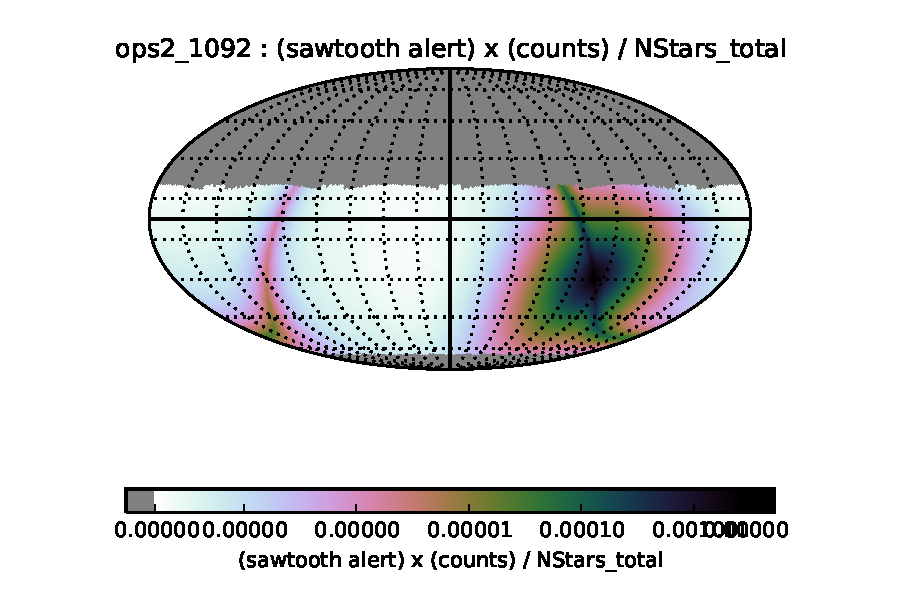
\includegraphics[width=7cm]{./figs/milkyway/galacticSN_SkyMap_1092.pdf}
  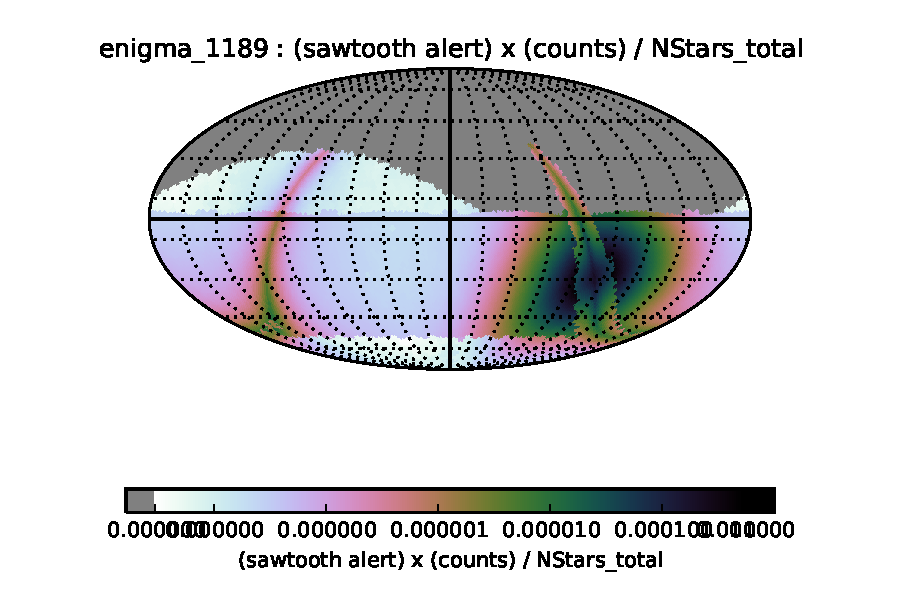
\includegraphics[width=7cm]{./figs/milkyway/galacticSN_SkyMap_1189.pdf}
%  \includegraphics[width=6cm]{./figs/milkyway/galacticSN_Histogram_1092.pdf}
%  \includegraphics[width=6cm]{./figs/milkyway/galacticSN_Histogram_1189.pdf} 
  \caption{\new{Figure of merit $FoM_{preSN}$~describing LSST's sensitivity to any pre-Supernova outburst, broken down by sightline, as sky-maps. $FoM_{preSN}$~is estimated for two OpSim runs (to-date); ops2-1092 (left) and enigma-1189 (right). The normalizing factors $N_{\ast, total}$ are $1.120\times 10^{12}$~for ops2-1092 and $1.121 \times 10^{12}$~for enigma-1189. The imprint of reduced sampling towards the inner plane can be clearly seen for enigma-1189.}}
\end{center}
\label{f_opSim_GalacticSN}
\end{figure}


%The current baseline cadence (${\tt enigma\_1189}$) partially excludes the Galactic Plane from the% deep-wide-fast survey and instead adopts a 
%nominal 30 visits per filter as part of a special proposal. We have proposed an OpSim run that inc%ludes the Galactic Plane in the 
%deep-wide-fast survey:

%\url{https://github.com/LSSTScienceCollaborations/ObservingStrategy/blob/master/opsim/Proposal_GP.md}

% The Figures of Merit listed above must now be implemented and applied to the OpSim databases.

%The metrics listed above should be carefully compared between our proposed run and the baseline cadence.


% --------------------------------------------------------------------

\subsection{Discussion: required work}
\label{sec:\secname:MW_Disk_discussion}

The Figures of Merit listed above must now be implemented within the
sims\_maf framework and applied to representative science
cases. \new{See Table \ref{tab_SummaryMWDisk} at the end of this subsection for initial
  efforts along these lines.}

We welcome input and volunteers for this effort. 

Qualitatively, however, we can note immediately that the current
baseline cadence (${\tt enigma\_1189}$) partially excludes the
Galactic Plane from the deep-wide-fast survey and instead adopts a
nominal 30 visits per filter as part of a special proposal - which
also tends to cluster the visits in the inner Plane within the first
few years of the survey. This already seriously compromises the time
baseline (see figure 4.3 of Section
\ref{sec:MW_Astrometry:MW_Astrometry_OpSim} for a demonstration applied to
proper motions).

We have proposed an OpSim run that includes the Galactic Plane in the
deep-wide-fast survey:

\url{https://github.com/LSSTScienceCollaborations/ObservingStrategy/blob/master/opsim/Proposal_GP.md}

\begin{table}
  \begin{tabular}{l|p{6cm}|c|c|c|c|p{5cm}}
    FoM & Brief description & {\rotatebox{90}{enigma-1189}} & {\rotatebox{90}{ops2-1092}} & {\rotatebox{90}{future run 1}} &  {\rotatebox{90}{future run 2}} & Notes \\
    \hline
    1.1 & \footnotesize{LMXB ellipsoidal variations}      & - & - & - & - & - \\
    1.2 & \footnotesize{Uncertainty in dwarf nova duty cycle}   & - & - & - & - &  \footnotesize{LSST as initial trigger} \\
    2.1 & \footnotesize{Fraction of Novae detected}       & - & - & - & - &  - \\
    3.1 & \footnotesize{Galactic Supernova pre-variability} & 0.25 & {\bf 0.85} & - & - & \footnotesize{Fraction of SN2010mc-like outbursts that LSST would detect; $FoM_{preSN} = f_{var} \times N_{\ast}$} \\
    4.1 & \footnotesize{Fraction of triggered microlens candidates} & - & - & - & - & - \\
    4.2 & \footnotesize{Uncertainty in disk-disk microlens distribution parameters due to missed events} & - & - & - & - & \footnotesize{LSST as initial microlens trigger} \\
    5.1a & \footnotesize{Median (over sight-lines) of the uncertainty in $E(B-V)$} & - & - & - & - & \footnotesize{(Most useful FoM probably a spatial map of the uncertainty.)} \\
    5.1b & \footnotesize{Variance (over sight-lines) of the uncertainty in $E(B-V)$} & - & - & - & - & - \\
  \end{tabular}
\caption{Summary of figures-of-merit for the Galactic Disk science cases. The best value of each FoM is indicated in bold.}
\label{tab_SummaryMWDisk}
\end{table}


%Discussion: what risks have been identified? What suggestions could be
%made to improve this science project's figure of merit, and mitigate
%the identified risks?



% ====================================================================

\navigationbar

% ====================================================================
%+
% SECTION:
%    section-name.tex  % eg lenstimedelays.tex
%
% CHAPTER:
%    chapter.tex  % eg cosmology.tex
%
% ELEVATOR PITCH:
%    Explain in a few sentences what the relevant discovery or
%    measurement is going to be discussed, and what will be important
%    about it. This is for the browsing reader to get a quick feel
%    for what this section is about.
%
% COMMENTS:
%
%
% BUGS:
%
%
% AUTHORS:
%    Phil Marshall (@drphilmarshall)  - put your name and GitHub username here!
%-
% ====================================================================

\section{Star Formation History of the Milky Way}
\def\secname{MW_SFH}\label{sec:\secname} % For example, replace "keyword" with "lenstimedelays"

\credit{pmmcgehee}

\label{sec:\secname:targets}

% This individual section will need to describe the particular
% discoveries and measurements that are being targeted in this section's
% science case. It will be helpful to think of a ``science case" as a
% ``science project" that the authors {\it actually plan to do}. Then,
% the sections can follow the tried and tested format of an observing
% proposal: a brief description of the investigation, with references,
% followed by a technical feasibility piece. This latter part will need
% to be quantified using the MAF framework, via a set of metrics that
% need to be computed for any given observing strategy to quantify its
% impact on the described science case. Ideally, these metrics would be
% combined in a well-motivated figure of merit. The section can conclude
% with a discussion of any risks that have been identified, and how
% these could be mitigated.

LSST gives the opportunity to survey extensive areas
around star formation regions in the Southern hemisphere. Among
others, it would allow to study the Initial Mass Function down to the
sub-stellar limit across different environments. Young stars are
efficiently identified by their variability.

Section 8.10.2 in the LSST Science Book (p298--299) provides a
  thorough scientific motivation for the characterization of young
  stars through variability, including discussion of the observational
  signatures of the diverse physical phenomena driving observed time
  variability. The general observable is strong, irregular flaring
  across the entire $ugrizy$~bandpass of LSST. Flaring can last from
  minutes to years, and at amplitudes from a few tenths to several
  magnitudes.

% WIC - the following para has been removed since it's already present
% verbatim at the end of Section 8.10.2 in the LSST Science Book.

%LSST will increase the sample size for detailed follow-up observations
%due its ability to survey star formations at large heliocentric
%distances and to detect variability in embedded and highly extincted
%young objects that would otherwise be missed in shallower
%surveys. During its operations LSST will also provide statistics on
%the durations of high states, for at least one important tracer
%population (the shorter-duration EXor variables).

% --------------------------------------------------------------------

\subsection{Target measurements and discoveries}
\label{sec:\secname:targets}

The nature of the variability in young stars changes with evolutionary
status. For the youngest stars still undergoing significant mass
accretion, FU Orionis and related outbursts can occur due to
circumstellar disk instabilities. As the natal environment dissipates
and the accretion rates drops, the stars take on a Classical T Tauri
appearance where the variability is primarily due to changes in the
accretion flow and rotational modulation of hot spots resulting from
accretion shocks on the protostellar photosphere. Also present are the
signature of cool spots arising from strong magnetic fields. This cool
spot rotational modulation is responsible for the variability in the
disk-less, and older, weak-line T Tauri stars.

Of particular interest are the FUor and EXor variables, which are
  named after the prototype objects FU Orionis \citep{hartmann96}
  and EX Lupi \citep{herbig01} respectively, and for which
  only a relatively small number of examples are known. In these
  pre-main sequence objects, eruptive outbursts of up to 6 magnitudes
  have been observed, with high state durations from years to
  decades. In addition to triggering follow-up observations, LSST
  should be able to set the first population constraints on the
  duration of high states, particularly for the short end of the
  timescale distribution for these eruptive variables.


% \new{(WIC: Material already in LSST Science Book removed.)}


%{\bf CTTS and WTTS material goes here.}

%Here are the references cited above:\\
%Hartmann \& Kenyon 1996, ARA\&A, 34, 207 \\
%Herbig et al. 2001, PASP, 113, 1547 \\
%Herbig 1977, ApJ, 217, 693 \\
%Aspin et al. 2009, ApJ, 692L, 67 \\
%Hodapp et al. 1996, ApJ, 468, 861 \\
%McGehee et al. 2004, ApJ, 616, 1058 \\


%Describe the discoveries and measurements you want to make.

%Now, describe their response to the observing strategy. Qualitatively,
%how will the science project be affected by the observing schedule and
%conditions? In broad terms, how would we expect the observing strategy
%to be optimized for this science?


% --------------------------------------------------------------------

\subsection{Metrics}
\label{sec:\secname:metrics}

In order to assess the ability of LSST to 1) identify and 2) classify
Young Stellar Objects we need to quantify the variability timescales
and amplitudes of both Class I/II (stars with disks, including
Classical T Tauris) and Class III (Weak-line T Tauris).  Inclusion of
eruptive variables (FUor/EXor) is appropriate as well.

In brief, Weak-line T-Tauris are quasi-periodic with amplitudes of 0.1
to 0.3 mag and periods 1 to $\sim$15 days, so their variability is
comparable to that of $\gamma$ Dor stars. Given the temporal evolution
of cool spots, a period recovery analysis such as shown for RR Lyrae
stars is likely difficult.  The embedded systems and Classical T
Tauris are irregular variables but have been shown to have distinctive
colors due to extinction and the ultraviolet and blue excess arising
from accretion shocks.

Table \ref{table:pseudoForExor} shows a possible Figure of Merit for the recovery by LSST of the distribution of EXor high-state duration in outburst.

% --------------------------------------------------------------------

%\subsection{OpSim Analysis}
%\label{sec:\secname:analysis}

%OpSim analysis: how good would the default observing strategy be, at
%the time of writing for this science project?

\begin{table}
\small
\begin{tabular}{c p{12cm}}
& {\it Figure of Merit for recovery of EXor high--state duration distribution}\\
\hline
1.  & Produce ASCII lightcurve for eruptive outburst \\
2.  & Initialise large array to store the maps of fraction detected as a function of duration and amplitude. \\
2.  & for {\it duration T} in range \{min, max\}:  \\
3.  & ~~~~ for {\it amplitude A} in range \{min, max\}: \\
4.  & ~~~~~~~~~~ run {\tt mafContrib/transientAsciiMetric} \\
5.  & ~~~~~~~~~~ store the spatial map of the fraction detected for this (A, T) pair \\
6.  & Initialise master arrays to hold the run of duration distribution measurements.\\
7. & Produce distribution of high--state durations and amplitudes from which the simulations will be drawn. \\
8.  & for {\it iDraw} in range \{1, nDraws\}:\\
9.  & ~~~~ construct model population with input duration distribution \\
10.  & ~~~~ Apply the stored metrics from 2-5 to measure fraction recovered \\
11.  & ~~~~ Characterize the duration distribution for this draw \\
12. & ~~~~ Fill the {\it iDraw}'th entry in the master arrays. \\
13. & {\bf FoM 1:} Compute the median and variance of the upper/lower quintiles. \\
14. & {\bf FoM 2:} Evaluate the bias between recovered and input high-state duration. \\
\hline
\end{tabular}
\caption{\new{Steps for Figure of Merit recovering the distribution
  for the duration of EXor high states. See Section \ref{sec:MW_SFH:targets} }}
\label{table:pseudoForExor}
\end{table}



% --------------------------------------------------------------------

\subsection{Discussion}
\label{sec:\secname:discussion}

Galactic star formation regions are largely found at low Galactic
latitudes or within the Gould Belt structure. As such study of young
stars with LSST is closely tied to other science goals concerning the
Milky Way Disk and is subject to the concerns of both crowded field
photometry and the observing cadence along the Milky Way.

The embedded and Classical T Tauri stars also undergo significant and
rapid color changes due to accretion processes. The ability of LSST to
track these variations in color could be limited by the interval
between filter changes.

% ====================================================================

\navigationbar

% ====================================================================
%+
% SECTION:
%    section-name.tex  % eg lenstimedelays.tex
%
% CHAPTER:
%    chapter.tex  % eg cosmology.tex
%
% ELEVATOR PITCH:
%    Explain in a few sentences what the relevant discovery or
%    measurement is going to be discussed, and what will be important
%    about it. This is for the browsing reader to get a quick feel
%    for what this section is about.
%
% COMMENTS:
%
%
% BUGS:
%
%
% AUTHORS:
%    Phil Marshall (@drphilmarshall)  - put your name and GitHub username here!
%-
% ====================================================================

\section{Dust in the Milky Way}
\def\secname{MW_Dust}\label{sec:\secname} % For example, replace "keyword" with "lenstimedelays"

\noindent{\it Peregrine M. McGehee} % (Writing team)

% This individual section will need to describe the particular
% discoveries and measurements that are being targeted in this section's
% science case. It will be helpful to think of a ``science case" as a
% ``science project" that the authors {\it actually plan to do}. Then,
% the sections can follow the tried and tested format of an observing
% proposal: a brief description of the investigation, with references,
% followed by a technical feasibility piece. This latter part will need
% to be quantified using the MAF framework, via a set of metrics that
% need to be computed for any given observing strategy to quantify its
% impact on the described science case. Ideally, these metrics would be
% combined in a well-motivated figure of merit. The section can conclude
% with a discussion of any risks that have been identified, and how
% these could be mitigated.

Interstellar dust is a significant constituent of the Galaxy. Its composition and associated extinction
properties tell us about the material and environments in which stars and their planets are formed.
Dust also presents an obstacle for a wide-range of astronomical observations, causing light from
stars in the plane of the Milky Way to be severely dimmed and causing the apparent colors of
objects observed in any direction to be shifted from their intrinsic values. These color shifts
are dependent upon the dust column density along the line of sight and the radiative transport
properties of the dust grains.

The wavelength dependence of the absorption due to dust is parametrized in the widely used model
of Cardelli et al. (1989) by the ratio of general to selection extinction in the Johnson B and V
bands, defined as RV = AV /E(B − V ). The value of RV depends on the dust composition and
grain size along the line of sight. In the low-density diffuse ISM, RV has a value ∼ 3.1, while in
dense molecular clouds, RV can be higher with values 4 < RV < 6.

The fundamental importance of a well-characterized dust map to astronomy is underscored by the
> 5, 000 citations to the dust and extinction maps by Schlegel et al. (1998), henceforth SFD98.
The SFD98 maps are based on far-infrared observations and predict reddening in specific bands by
assuming a dust model and RV = 3.1 as appropriate for sky areas away from the Galactic plane.
Despite the great contribution that the SFD98 extinction map has made to the field, these maps
suffer from several issues that limit their utility in some regimes of study. 1) While the SFD98
map seems to be well calibrated at low column density, various tests using galaxy counts, star
counts and colors, and stellar spectrophotometry indicate that SFD98 overpredicts dust by ∼ 30%
above E(B − V ) ∼ 1 mag. Because this overcorrection appears especially in cold clouds, it is
likely related to the temperature correction adopted in the SFD98 model. 2) In some cases,
especially at low Galactic latitudes, RV variation is important and is not tracked by SFD98. 3)
For study of low-redshift, large-scale structure, contamination by unresolved point sources can be
important (see Yahata et al. 2007). 4) Finally, the resolution of the SFD98 map is ∼ 60, which
is larger than the angular scales subtended by nearby, resolved, galaxies for which a carefully
characterized foreground dust distribution is particularly important. For all these reasons, LSST
stellar photometry, which can constrain the temperature correction, overall calibration, and point
source contamination of SFD98, is valuable.

For the study of stellar populations and objects within the Galactic disk it is also important to
determine both the line of sight extinction and the value of RV at a specific distance, neither of
which is dealt with by SFD98. By analysis of the observed reddening of stellar colors, we will verify
both the dust column density and RV values predicted by these maps and can also determine the
local spatial distribution of the dust. We will do this utilizing two specific stellar populations - the
M dwarfs and the F turn-off stars.

The reddening of stellar colors due to the presence of interstellar dust along the line of sight can,
in principle, be used to map the three-dimensional distribution of that dust. This requires that
two important parameters are determined - the amount the observed stellar color is reddened and
the distance to the star. By comparison of the color excess measured in stars at varying distances
we can infer the location of the extincting medium. However, given lack of an a priori knowledge
of the light of sight extinction, which is the very quantity we wish to measure, it can be difficult
to accurately assign intrinsic stellar colors and luminosities in order to determine the amount of
color excess and the distance. This difficulty can be surmounted, however, if we utilize reddeninginvariant
combinations of colors whose values can be used to infer location on the stellar locus
and hence intrinsic colors and luminosities. This technique is viable if we use LSST photometry of
M dwarfs as the stellar locus in ugriz colors is nearly parallel to the reddening vector for all but
coolest stars.


% --------------------------------------------------------------------

\subsection{Target measurements and discoveries}
\label{sec:\secname:targets}

The use of stellar samples to create three-dimensional extinction maps has an established history
beginning with the work of Neckel & Klare (1980); however these, including studies based on SDSS
photometry, are typically limited to heliocentric distances of 1−2 kpc. In the full co-added survey,
LSST will be able to map dust structures out to distances exceeding 15 kpc, thus revealing a
detailed picture of this component of the Milky Way Galaxy.

Mapping of the dust component of the Galactic ISM requires detection of the reddening in the
colors of stars at known distances. The reddening is determined from the color excess deduced
by comparison of the observed colors with those expected based on the stellar spectral type. In
the absence of identifying spectra, the spectral type can be inferred by dereddening the observed
colors (assuming a specific extinction law, i.e., a particular value of RV ) back to the unreddened
stellar locus in a color-color diagram. This dereddening is equivalent to assignment of reddeningfree
colors along the stellar locus, which measure the location in the color-color diagram along
the direction perpendicular to the reddening vector. Once the effective line of sight reddening has
been computed, the distance to each star can be determined using dereddened photometry and
well-calibrated color-absolute magnitude relations.


Reddening-invariant Indices

Reddening-free colors were defined in the SDSS ugriz system by McGehee et al. (2005) for characterization
of embedded pre-main sequence stars and were subsequently used as part of the SDSS
photometric quality analysis system (Abazajian et al. 2009). The general definition is
Qxyz = (x − y) − (y − z) ×
E(x − y)
E(y − z)
(7.1)
where (x − y) and (y − z) are the colors used to construct the color-color diagram. This extends
the definition by Johnson & Morgan (1953) whose original Q would be defined here as QUBV . The
reddening coefficients adopted by the SDSS (Stoughton et al. 2002) follow SFD98 and assume the
“standard” dust law of RV = 3.1 and a z = 0 elliptical galaxy spectral energy distribution.
In Figure 7.4 we compare the variation of the three reddening-invariant indices formed from the
ugriz passbands (Qugr, Qgri, and Qriz) with g − i, a proxy for stellar spectral type (Covey et al.
2007). For g − i < 1.9 (spectral type earlier than M0) there is little variation in any of these
indices, indicating that the stellar locus is approximately parallel to the reddening vector in the
corresponding color-color diagrams. For the M dwarfs we see that the Qgri has the largest range
between M0 and M5, and thus is of the greatest utility for determination of spectral type.
213

Selection of Reddening Probes

For determination of spectral type and intrinsic stellar colors to be accurate, the stars used as
reddening probes must reside on the portion of the stellar locus that is not aligned with the
reddening vector in a color-color diagram. As we have seen, this condition is fulfilled by stars of
spectral types M0 and later. In the final panel of Figure 7.4 we show the criteria used to select
for early and mid M dwarfs based on the Qgri and Qriz indices, where the latter is used to filter
out earlier and more luminous background stars whose Qgri colors are similar to M0 dwarfs. The
threshold at M5 is chosen to remove the later spectral type stars, which are too intrinsically faint
to serve as probes for all but the nearest dust structures.

Analysis of the LSST imaging data will adapt the following procedure as used in the SDSS High
Latitude Cloud Survey (McGehee 2009):
• The intrinsic g − i color ((g − i)0) is determined from the observed Qgri color based on a
fifth-order polynomial fit using the median stellar locus (Covey et al. 2007) and assuming
RV = 3.1.
• The total reddening to each star is computed from the g − i color excess.
• Distances are assigned based on the color-absolute magnitude relations of Ivezi´c et al. (2008)
using the dereddened photometry.
• E(B − V ) maps are created at specific distance ranges using the adaptive technique of
Cambr´esy et al. (2005) in which the reddening at each pixel is the median of that computed
for the N nearest extinction probes.

Example maps from the SDSS project are depicted in Figure 7.5 for a 10◦ by 10◦ field containing the
high latitude molecular cloud HRK 236+39. These maps are based on the reddening computed for
stars having distance moduli of 7.0 < m − M < 8.0, 8.0 < m − M < 9.0, and 9.0 < m − M < 10.0.
The reddening shown at each pixel is computed as the median of the E(B − V ) values obtained
for the N = 5 nearest stars. The reddening associated with the HRK 236+39 cloud is discernible
at m − M > 7.0 (d > 250 pc) and is obvious at m − M > 8.0 (d > 400 pc).

Distance and AV Limits

It has been demonstrated that accurate three-dimensional mapping of the local ISM within a few
kpc is possible using SDSS photometry of M dwarfs (McGehee 2009). Analysis of the g − i color
excess in regions effectively free of interstellar reddening shows that distance modulus limits of 7.0
(at M5) to 11.2 (at M0) result in a volume-limited survey nearly free of the systematic color biases
inherent in this g-band limited data set.

These limits correspond to g ∼ 20.6 and σg ∼ 0.02−0.03 for single-epoch SDSS observations. Given
the relative g-band 5 σ limits of SDSS and the LSST single epoch and final co-added surveys, we
estimate that the the co-added LSST data will reach 5 magnitudes deeper in m-M, allowing the
LSST to probe dust structures across a significant portion of the Galaxy. In Figure 7.6 we depict
the portion of the Galactic disk accessible by the LSST single and co-added surveys as well as the
SDSS assuming the vertical and radial scale height dust model outlined in § 3.7.1.

7.5.2 Variation in Extinction Laws

Changes in the absorption properties of dust grains, as parametrized by RV , result in a shift in
both the direction and length (for a specific dust column density) of the reddening vector in a
color-color diagram. This is reflected in the reddening-free colors by variations in the scaling factor
used when defining the linear combination of colors, e.g., in the E(g − r)/E(r − i) term for Qgri.
By analysis of the observed color shifts due to reddening it is possible to constrain the value of RV
along the line of sight and gain insight into the nature and composition of the interstellar dust in
that region of the Galaxy.

The LSST will be in a unique position to measure the changes in the observed reddening vector
due to RV variations due to its superb photometric accuracy (see § 2.6). The specifications for
LSST are a factor of two more stringent than typically achieved in previous surveys, including the
SDSS (except for limited photometric conditions).

F turn-off stars (gabs ∼ 4) reside on the blue tip of the stellar locus in ugriz color space and for
g > 19 trace the total Galactic extinction along high-latitude lines of sight. This method will
provide a verification of the far-infrared-based SFD98 extinction model and allow study of the
variations in dust grain sizes as inferred from RV . The value of RV provides a general indicator of
grain size, with the RV ∼ 4.5 − 5 values seen in star formation regions suggestive of grain growth
in cold molecular clouds.

The slope of the reddening vector is sensitive to the value of RV as shown in Figure 7.7. For the
SDSS passbands and an assumed F star source SED, the value of E(u−g)/E(g−r) is larger for small
RV and decreases with a slope of approximately −0.11 with increasing RV . This analysis mandates
precise and well-calibrated photometry. For example, determination of RV to within σRV = 0.5
requires the slope of the reddening vector to be measured to σm = 0.06. If E(B −V ) = 1 along the
line of sight, then the required photometric accuracy is 2%. The photometric accuracy requirement
becomes proportionally more stringent as the dust column density decreases due to the reduced
movement of the blue tip in the color-color diagram. LSST, with better than 1% photometric
accuracy in the final co-added survey, will be able to study RV variations in both Galactic plane
and high latitude environments.
Describe the discoveries and measurements you want to make.

Now, describe their response to the observing strategy. Qualitatively,
how will the science project be affected by the observing schedule and
conditions? In broad terms, how would we expect the observing strategy
to be optimized for this science?


% --------------------------------------------------------------------

\subsection{Metrics}
\label{sec:\secname:metrics}
 From the material in the science book and what you have contributed, I think a metric dependent on the photometric accuracy metrics might be the way to go (e.g. estimate the error in A_V and E(B-V) for different strategies, which would be a simple scaling for each pixel in the spatial map given the nominal scalings with exposure time in each filter).

The spacing in time of the visits doesn't matter for dust (as far as I know). 
Pushing to fainter magnitudes (which means both better seeing and longer exposures) matters, both because we want more stars, and in particular, we want more stars *behind* the dust.  If we can't see through the dust, we can't do much.  At PS1 depth, we get to ~ 3-5 kpc, with maybe up to 1ish mag E(B-V).  If we went 3 or 4 mags fainter, how far could we go?  This is a good question, and one I am unlikely to answer by next week.  But it is something we should figure out. 

I'm cc'ing Greg in case he has a better answer, or in case he has some mock map runs that give us an idea of how our results depend on survey depth. 
Quantifying the response via MAF metrics: definition of the metrics,
and any derived overall figure of merit.

{\bf Metric 1: Uncertainty and bias in $E(B-V)$~estimates as a
  function of location on-sky.} Dependencies:

\begin{itemize}
  \item Stellar population throughout the survey (e.g. Knut / Peter developments; TRILEGAL?);
    \item Dust map throughout the survey region;
    \item Scale photometric error predictions for each band from program requirements per exposure;
      \item Produce formal estimate on the error in extinction and reddening as a function of position on-sky within the survey.
\end{itemize}


% --------------------------------------------------------------------

\subsection{OpSim Analysis}
\label{sec:\secname:analysis}

OpSim analysis: how good would the default observing strategy be, at
the time of writing for this science project?


% --------------------------------------------------------------------

\subsection{Discussion}
\label{sec:\secname:discussion}

Discussion: what risks have been identified? What suggestions could be
made to improve this science project's figure of merit, and mitigate
the identified risks?


% ====================================================================

\navigationbar

% ====================================================================
%+
% SECTION:
%    MW_Astrometry.tex
%
% CHAPTER:
%    galaxy.tex
%
% ELEVATOR PITCH:
%
%-
% ====================================================================

\section{Astrometry with LSST: Positions, Proper Motions, and Parallax}
\def\secname{MW_Astrometry}\label{sec:\secname}

\credit{dgmonet}, \credit{DanaCD}, \credit{jgizis}, \credit{mliu},
\credit{caprastro}, \credit{willclarkson}, \credit{yoachim}

A number of Milky Way science cases of interest to the Astronomical
community will depend critically on the astrometric accuracy LSST will
deliver. While ``astrometry'' is not a science case in the framework
of this white paper, LSST's astrometric performance will be sensitive
to the particular choice of observing strategy.
%While astrometry is not a science case, high astrometric accuracy enables
%a large number of science cases.
Hence, the LSST Observing Strategy needs to be examined for systematic
trends that might limit or even preclude precise measures of
stellar positions, proper motions, parallaxes, and perturbations that
arise from unseen companions.

\autoref{sec:\secname:MW_Astrometry_measurements} highlights two
science cases at opposite scales of distance from the Sun that require
accurate and precise astrometry and/or proper motion
measurements. \autoref{sec:\secname:MW_Astrometry_metrics} presents
Metrics for LSST's astrometric performance, and discusses Figures of
Merit for the two highlighted science cases. These metrics are applied to two example OpSim runs in
\autoref{sec:\secname:MW_Astrometry_OpSim}. Finally in Section
\ref{sec:\secname:MW_Astrometry_furtherwork}, the work that is still
needed is discussed, both in terms of the Metrics and the Figures of
Merit that depend on them.

%Each of these cases stresses different aspects of the LSST hardware, software,and observing strategies.

%, here we highlight three representative science cases.
%that illustrate the various impacts of the observing strategy might
%be:
%To highlight the
%various astrometric impacts of the strategy, three science cases have
%been chosen for particular attention:

%\subsection{Introduction: Astrometry as a special case}
%\label{sec:\secname:MW_Astrometry_intro}

\subsection{Target Measurements and Discoveries}
\label{sec:\secname:MW_Astrometry_measurements}

%\begin{itemize}
%\item[1.] Identification of Streams in the Galactic Halo using proper motions.
%\item[2.] A complete sample of stars in the solar neighborhood.
%\end{itemize}
%\item The tie between the Radio and Optical realizations of the International Celestial Reference System.
%\item The specific and ensemble agreement between LSST and Gaia parallaxes.

{\bf 1. Identification of Streams in the Galactic Halo Using Proper Motions}

Much of the Milky Way's stellar halo was built by the accretion of smaller galaxies. Given that these galaxies
were generally of low mass, their tidal debris should still form coherent structures in phase space, especially
in the outer Galaxy where dynamical times are long. The identification of these streams would allow
a reconstruction of the accretion history of the Milky Way. Tides also lead to the dissolution of globular clusters,
leaving notably thin streams that serve as sensitive tracers both of the Galactic potential and of the presence of dark
subhalos.

A relatively small number of streams, originating from both dwarfs and globular clusters, have been identified via photometry
of individual stars in large surveys such as SDSS\@. However, only the highest surface brightness structures can be found
in this manner, and it is often difficult to trace the streams over their full extent. LSST will enable streams to be identified
by stellar proper motions, and combined with targeted follow-up spectroscopy, will yield full 6-D position and velocity measurements suitable for dynamical modeling.
Further, it will allow the discovery of tidal debris that is no longer spatially coherent but which can be unambiguously identified in phase space.

Finally, streams and other kinematically-distinct halo substructure
can be identified and characterized by combining proper motions and
photometry in reduced proper-motion diagrams \citep[e.g.,][]{carlin12},
and by analyzing proper-motions of tracers such as
RR Lyrae and giants over large portions of the sky \citep[e.g.,][]{casettidinescu15}.

{\it Response to observing strategy:} Most stars in streams will be main-sequence stars, and the old main sequence turnoff  is located at $r\sim24$ at a distance of 100 kpc.
The nominal LSST proper motion precision at this magnitude is 1 mas yr$^{-1}$, corresponding to about 475 km s$^{-1}$ at this distance. The proper motion
measurements will be better for brighter stars, but in general ensembles of stars will be necessary for accurate measurements. To make accurate proper motion measurements for faint stars, several key components are required. First, a zero point must be established, possibly via background galaxies located in each field. Next, the observations must cover a sufficient range of epochs to reliably detect linear proper motions.

To identify streams over their full lengths of many degrees of the sky, relative astrometry over small fields will not be sufficient. Therefore the absolute astrometric frame is important. Matching the optical astrometry to the radio International Celestial Reference System (ICRS) relies on measuring accurate positions for objects visible in both wavelength regimes.
These are typically distant QSOs. Unfortunately, many QSOs have detectable optical or radio structures that degrade the positions or suggests a displacement between the location of the sources of the radio and optical radiation. LSST will need to identify a large number of point-like QSOs based on their colors and variability.

Since the number of galaxies is overwhelming toward faint magnitudes,
these must be exploited to produce a reliable absolute
proper-motion zero point. By using Gaia stars at the bright end
as absolute proper-motion calibrators we can quantify the precision
and accuracy of background galaxies as a secondary link to an inertial reference system, and thus improve the calibration at the faint end of the survey.

%The tie between the radio and optical reference frames relies on measuring accurate positions for objects visible in both wavelength regimes.  Whereas there are optical variable stars with radio emission, most have associated optical nebulosity that degrades the accuracy of the optical positions. The typical radio+optical object is a QSO.  Unfortunately, many QSOs have detectable optical or radio structures that degrade the positions or suggests a displacement between the location of the sources of the radio and optical radiation.  The major contribution from LSST will be the identification of a large number of QSOs based on their colors that have minimal (if any) spatially extended structure.  The impact of this search has no obvious impact on the cadence other than temporal coverage to identify variability.

{\bf 2. A Complete Sample of Stars in the Solar Neighborhood}

The direct solar neighborhood offers our only chance to get make a complete sample of stars, brown dwarfs, and stellar remnants that encompass the entire formation and dynamical history of the Milky Way. While Gaia will offer parallax measurements for perhaps billions of stars, its faint magnitude limit of $G\sim 20$ will limit its measurements of the lowest-mass objects
and remnants to nearby objects, much less than the thin disk scale height of $\sim 300$ pc. For example, Gaia can only measure parallaxes for $0.2 M_{\odot}$ M dwarfs to about 100 pc
and $0.1 M_{\odot}$ M dwarfs to only \emph{10 pc}, showing that Gaia is ill-suited for studies of the coolest dwarfs. By contrast, LSST can measure parallaxes for $> 10^5$ M dwarfs and thousands of L/T brown dwarfs (the coolest Y dwarfs are too faint even for LSST; little contribution is likely here beyond the sample provided by WISE). Gaia will likewise be limited to cool white dwarfs within $\sim 100$ pc with which to estimate the age of the disk, and the thick disk and halo will be out of reach. LSST can directly compare white dwarf luminosity functions to determine precise differential ages for the thin disk, thick disk, and halo.

{\it Response to observing strategy:} Successfully completing this project will require parallax measurements much fainter than possible with Gaia as well as a verification that the LSST and Gaia parallax measurements are consistent in the overlapping magnitude range.

The measurement of stellar parallax puts the substantial constraints on the observing cadence. There are two major issues: the need to sample a wide range of parallax factor (related to time of year), and breaking the correlation between differential color refraction and parallax factor.

``Parallax factors" characterize the ellipse of the star's apparent motion as seen over the course of a year. The shape of the ellipse is given by the Earth's orbit and is not a free parameter in the astrometric solution. The amplitude of the right ascension parallax factor is close to unity while the amplitude of the declination parallax factor is dominated by the sine of ecliptic latitude.
The right ascension parallax factor has maximum amplitude when the star is approximately six hours from the Sun, so the optimum time for parallax observing is when the
star is on the meridian near evening or morning twilight. Atmospheric refraction displaces the star's apparent position in the direction of the zenith by an amount dependent on both the wavelength of the light and the distance to the zenith. Whereas the measured position of star is a function of the total refraction, the measurement of parallax
and proper motion depends on the differences in the refraction as a function of the color of each star and the circumstances of the observations.  This
dependence is called differential color refraction. The combination of parallax factor and differential color refraction leads to two rules: (i) Observations need to cover the widest possible range in parallax
factor, and (ii) The correlation between parallax factor and hour angle in the observations needs to be minimized.

%with respect to the meanmotion of the reference frame.

%The search for faint proper motion stars has two key components.  The first is the need to identify stars that move from the ensemble of other image features that can cause confusion.  For example, a compact group of stars that contains one or more stars of variable brightness can confuse the catalog correlation algorithm.  The other is the need to establish the zero point. For the case of relative astrometry, meaning the measurement of relative positions in an image, the question remains on how to remove the mean motion of the reference frame.  For example, astrometry on certain classes of galaxies might produce a zero point of sufficient accuracy.  This leads to a third constraint on the observing cadence.
% \begin{itemize}
%\item [3)] Observations must cover a sufficient range of epochs so that stars with
%linear or periodic motions can be identified at a high level of confidence.
%\end{itemize}


%\subsection{Sensitivity of parallax measurements to observing strategy}
%\label{sec:\secname:MW_Astrometry_cadence}

%\medskip


\subsection{Metrics and Figures of Merit for LSST's delivered astrometric accuracy}
\label{sec:\secname:MW_Astrometry_metrics}

%\medskip

First we discuss metrics for the observing strategy that affect all of
LSST's astrometric measurements, then discuss figures of merit for the
two science cases. (The three general metrics were identified years
ago and are already in the suite of MAF utilities, and they should be
reviewed prior to making final decisions. For this reason, in addition
to the Figures of Merit later in the chapter, we present spatial maps
and histograms for the metrics themselves in Section
\ref{sec:\secname:MW_Astrometry_OpSim}, for representative OpSim
strategies.)

\begin{itemize}
\item[A)] For each LSST field, the parallax factors at each epoch of
observation need to be computed.  The ensemble of these must be checked for
sufficient coverage of the parallactic ellipse.  In particular, the number of
measures with RA parallax factor less than --0.5 and greater than +0.5
needs to be tallied because these carry the most weight in the solution
for the amplitude (parallax).
\item[B)] For each LSST field,
%the hour angle of the observation needs to be
%computed, and
the correlation between hour angle and parallax factor
needs to be examined for significance.  The observing strategy must minimize
the number of fields with this correlation.
\item[C)] The epochs of observation for each field must be checked for a
reasonable coverage over the duration of the survey and to avoid
collections of too many visits during a few short intervals.
\end{itemize}

Within sims\_maf, metrics A (parallax factor distribution) and B
  (hour angle and parallax correlation) are implemented in a slightly
  different manner from the prescription above. We describe the
  implemented metrics here.

{\it Parallax factor coverage:} This is {\tt
    calibrationMetrics.ParallaxCoverageMetric} in sims\_maf. The
  inverse-variance weighted mean parallax offset is subtracted from
  the set of parallax offsets for an object at a given location with
  unit parallax amplitude, and the inverse-variance weighted mean
  $\langle r \rangle$~of the resulting residuals is returned, scaled
  to the range $0 \le \langle r \rangle \le 1$. For each measurement,
  the variance used in the weighting is the estimate of the
  (uncrowded) astrometric uncertainty returned by OpSim for a star of
  specified fiducial magnitude at the center of the HEALPIX of
  interest. What constitutes a ``good'' value for $\langle r \rangle$~depends on the location
  of the star in ecliptic co-ordinates. Near either ecliptic pole a
  star with uniform parallax coverage would have $\langle r \rangle
  \approx 1.0$~while on the ecliptic uniform coverage would produce
  $\langle r \rangle \approx 0.5$. For any location, $\langle r
  \rangle \approx 0$~would mean all the observations were taken with
  identical parallax factor and therefore any attempt to fit the
  parallax amplitude would be completely degenerate with the object's
  position.

{\it Parallax-Hour angle correlation:} This is metric {\tt
    calibrationMetrics.ParallaxDcrDegenMetric}. At the level of tens
  of milliarcsec, Differential Chromatic Refraction (DCR) shifts the
  apparent location of the star in a color-dependent manner. Depending
  on the hour-angle distribution of observations throughout the year,
  motion due to parallax can become degenerate with motion due to the
  pattern of DCR values sampled. This metric returns the Pearson
  correlation coefficient $\rho$~between the best-fit parallax
  amplitude and DCR amplitude, returning values in the range $-1.0 \le
  \rho \le +1.0$. The range of acceptable values for this metric is
  still under investigation; Monte Carlo simulation by one of us (DGM)
  suggests the parallax error becomes independent of
  $\rho$~(i.e. other effects dominate) for values $|\rho| \lesssim
  0.7$.



For the stream project discussed above, a simple to state (but perhaps complex to implement) figure of merit
is the number of streams that can be discovered in LSST via their proper motions. As a first
attempt, it would be reasonable to assume about 100 halo streams from old, metal-poor dwarf galaxies with
stellar masses $10^5-10^7 M_{\odot}$ distributed as $r^{-3.5}$. The stream widths and internal velocity
dispersions can be set from galaxy scaling relations, and their 3-D velocities consistent with a simple Galactic mass
model at their radii. Setting the stream lengths is more complicated, but should cover a large range from a few to many kpc.
Over a given area, the stream ``S/N" can roughly be taken as the number of stream stars (identified via proper motion, color, and magnitude)
divided by the square root of the number of field stars. For globular clusters, a similar number of streams could be included, but these should have much smaller widths (10s of pc)
and typical masses $10^4-10^5 M_{\odot}$. Eventually it would be desirable to use actual simulated stream parameters taken from cosmological models of the Milky Way (e.g.,
from the Aquarius simulation).

Solar neighborhood projects will be sensitive to the general parallax and proper motion metrics discussed above. More specific science figures of merit are {\it required} at this stage.  For example, the precision of the differential age measurement between the thin disk and halo, which would depend on the number of white dwarfs that can be isolated
from each population.

\subsection{OpSim Analysis}
\label{sec:\secname:MW_Astrometry_OpSim}

Here we present initial analysis of LSST's astrometric
performance. Two example strategies are assessed: the current baseline
strategy, \opsimdbref{db:baseCadence}, and the new cadence
\opsimdbref{db:NormalGalacticPlane}, which extends the Wide-Fast-Deep
survey to the Galactic Plane (see Section \autoref{sec:cadexp:alternatives}
for more detail on this run).

%the PanSTARRS-like cadence,
%\opsimdbref{db:opstwoPS}, which greater spatial uniformity and
%superior coverage of the Galactic Plane.

\subsubsection{Metrics: Parallax and proper motion precision}

Here we present the expected astrometric performance of LSST as a function of
location on-sky, for two main cuts on the survey strategies:
\begin{itemize}
  \item By time: objects detected in $g,r,i,z$, after years 1, 2 and 10
    of the survey (Figures \ref{fig_astrom_ByTime_PACoverage} -
    \ref{fig_astrom_ByTime_paError});
\item By filter: objects detected in $g,r,i,z$, or in $u$ only, or $y$ only, over the full 10 years of the survey (Figures~\ref{fig_astrom_ByFilter_PACoverage} - \ref{fig_astrom_ByFilter_paError}).
\end{itemize}

Astrometric performance for parallax is quantified using the following
metrics:
\begin{itemize}
  \item[1.] Parallax factor coverage (following metric A of \autoref{sec:\secname:MW_Astrometry_metrics}); values farther from 0 are better). See Figures \ref{fig_astrom_ByTime_PACoverage} \&  \ref{fig_astrom_ByFilter_PACoverage};
    \item[2.] Parallax-Hour angle correlation (metric B of \autoref{sec:\secname:MW_Astrometry_metrics}; values closer to 0 are better). See Figures \ref{fig_astrom_ByTime_PADegen} \& \ref{fig_astrom_ByFilter_PADegen};
      \item[3.] Proper motion error, for a star at apparent magnitude 21.0 in the filter specified (this addresses the distribution of measurement epochs, as recommended in Metric C in \autoref{sec:\secname:MW_Astrometry_metrics}; smaller values are better). See Figures \ref{fig_astrom_ByTime_pmError} \& \ref{fig_astrom_ByFilter_pmError};
        \item[4.] Parallax error, for a star at apparent magnitude 21.0 in the filter specified (smaller values are better). See Figures \ref{fig_astrom_ByTime_paError} \& \ref{fig_astrom_ByFilter_paError}.
\end{itemize}

{\it Limitations of the results presented in Figures \ref{fig_astrom_ByTime_PACoverage} to \ref{fig_astrom_ByFilter_paError}.:}
\begin{itemize}
  \item[i.] The spatial maps are clipped at $95\%$~in order to keep
    the color-scale at a sensible range; in some cases this has had
    the side effect of removing parts of the spatial coverage in the
    \opsimdbref{db:baseCadence} maps.

  \item[ii.] This analysis neglected spatial confusion in high-density regions. While this
    confusion would be the same whatever observing strategy was
    chosen, the measurement uncertainties for proper motion and parallax uncertainty
    should be regarded as lower limits.

    \item[iii.] The choice of fiducial apparent magnitude $r = u = y =
      21.0$~is arbitrary. It
      would be informative to repeat the analysis for a range of
      target apparent magnitudes that are better-matched to the
      specific science cases.

      \item[iv.] The comparison between single-filter and $griz$
        detections likely overestimates the measurement precision for
        the $u$-only and $y$-only detections, as an object only
        detected in a single filter may well not be detected in all
        images taken in that filter. While the comparison between
        filter subsets for a given strategy may therefore be highly
        approximate, the comparison between strategies for the same
        filter should be more reliable.

% WIC 2016-06-01 - item below removed, now that we are comparing two strategies with
% similar sky coverage.

%  \item[v.] We have not yet subdivided the samples by a meaningful
%    spatial co-ordinate (galactic latitude would be the obvious
%    choice). A large part of the breadth of the various metric values in
%    \opsimdbref{db:baseCadence} as compared to \opsimdbref{db:opstwoPS} may be
%      due to spatial nonuniformity of the sampling; replotting the
%      histograms coded by galactic latitude would be highly informative in this context.

\end{itemize}

{\it Indications at this date:} Despite these limitations, we note the following:

% WIC 2016-06-01 - updated for comparing wfdPlane to Baseline, not PanSTARRS-1 as was the case.

\begin{itemize}
  \item[I1.] Taking snapshots of the survey at various stages of completion (Figures \ref{fig_astrom_ByTime_PACoverage} -  \ref{fig_astrom_ByTime_paError}), strategy \opsimdbref{db:NormalGalacticPlane} is not significantly worse than \opsimdbref{db:baseCadence};
%\item[I2.] As might be expected, the distribution of metric values for the PanSTARRS-like cadence is narrower than for \opsimdbref{db:baseCadence} - thus astrometric survey uniformity is improved;
%\item[I2.] For the extremes of object color (objects detected only in the bluest or only in the reddest filter), the differences between strategies is weaker. The histogram of run \opsimdbref{db:baseCadence} still shows a population with poorer parallax measures (although this might be due to coverage of difficult-to-observe regions that are not covered at all by the PanSTARRS-like strategy).
\item[I2.] To first order, proper motion and parallax error are dominated by the total time coverage, as might be expected.
\end{itemize}

%% In the current incarnation, these will be big figures on the page. Consider
%% finding a way to summarize them!
\begin{figure}[ht]
  \begin{center}
  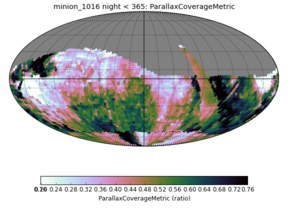
\includegraphics[width=2.0in]{./figs/milkyway/astromPanels/MW_Astrom_paCovge_Baseline_01y_map.png}
  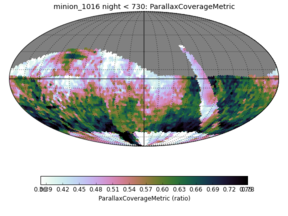
\includegraphics[width=2.0in]{./figs/milkyway/astromPanels/MW_Astrom_paCovge_Baseline_02y_map.png}
  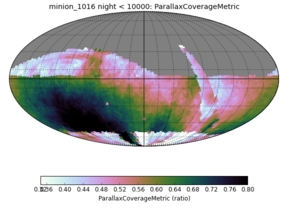
\includegraphics[width=2.0in]{./figs/milkyway/astromPanels/MW_Astrom_paCovge_Baseline_10y_map.png}
  \end{center}
  \begin{center}
  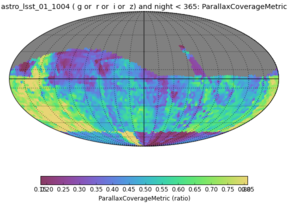
\includegraphics[width=2.0in]{./figs/milkyway/astromPanels/MW_Astrom_paCovge_wfdPlane_01y_map.png}
  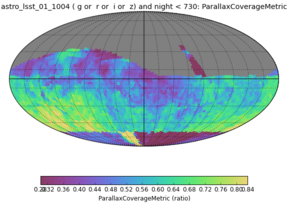
\includegraphics[width=2.0in]{./figs/milkyway/astromPanels/MW_Astrom_paCovge_wfdPlane_02y_map.png}
  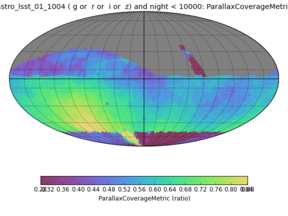
\includegraphics[width=2.0in]{./figs/milkyway/astromPanels/MW_Astrom_paCovge_wfdPlane_10y_map.png}
  \end{center}

  \begin{center}
  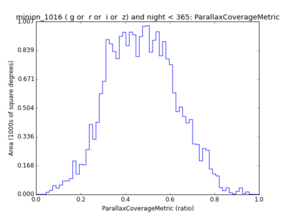
\includegraphics[width=2.0in]{./figs/milkyway/astromPanels/MW_Astrom_paCovge_Baseline_01y_hst.png}
  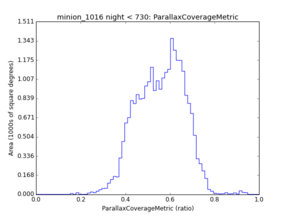
\includegraphics[width=2.0in]{./figs/milkyway/astromPanels/MW_Astrom_paCovge_Baseline_02y_hst.png}
  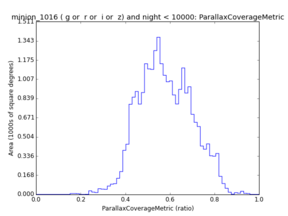
\includegraphics[width=2.0in]{./figs/milkyway/astromPanels/MW_Astrom_paCovge_Baseline_10y_hst.png}
  \end{center}
  \begin{center}
  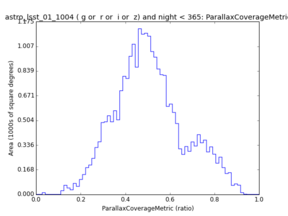
\includegraphics[width=2.0in]{./figs/milkyway/astromPanels/MW_Astrom_paCovge_wfdPlane_01y_hst.png}
  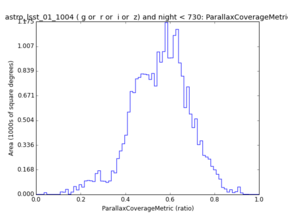
\includegraphics[width=2.0in]{./figs/milkyway/astromPanels/MW_Astrom_paCovge_wfdPlane_02y_hst.png}
  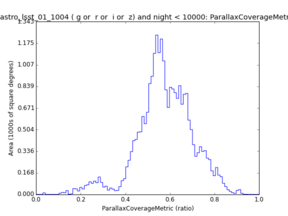
\includegraphics[width=2.0in]{./figs/milkyway/astromPanels/MW_Astrom_paCovge_wfdPlane_10y_hst.png}
  \end{center}
  \caption{Parallax coverage achieved at different epochs within the survey. {\it Top and Third row:} OpSim run \opsimdbref{db:baseCadence}. {\it Second and bottom row:} OpSim run \opsimdbref{db:NormalGalacticPlane} (wide-fast-deep extended to much of the inner Plane). Reading left-right, columns represent: {\it Left column:} all observations within the first 365 days of operation; {\it Middle column:} first two years; {\it right column:} the full 10-year survey. Spatial maps are clipped at 95\%, with histogram horizontal limits (0.0 - 1.0).}
  \label{fig_astrom_ByTime_PACoverage}
\end{figure}

\begin{figure}[ht]
  \begin{center}
  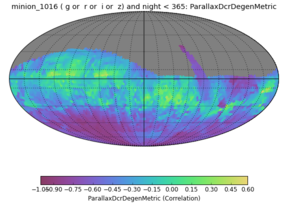
\includegraphics[width=2.0in]{./figs/milkyway/astromPanels/MW_Astrom_paDcrDegen_Baseline_01y_map.png}
  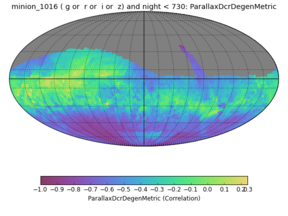
\includegraphics[width=2.0in]{./figs/milkyway/astromPanels/MW_Astrom_paDcrDegen_Baseline_02y_map.png}
  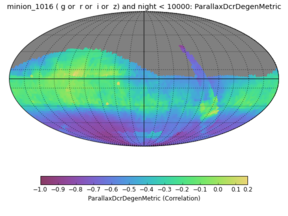
\includegraphics[width=2.0in]{./figs/milkyway/astromPanels/MW_Astrom_paDcrDegen_Baseline_10y_map.png}
  \end{center}
  \begin{center}
  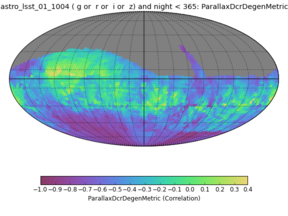
\includegraphics[width=2.0in]{./figs/milkyway/astromPanels/MW_Astrom_paDcrDegen_wfdPlane_01y_map.png}
  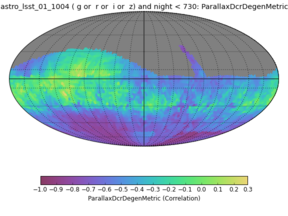
\includegraphics[width=2.0in]{./figs/milkyway/astromPanels/MW_Astrom_paDcrDegen_wfdPlane_02y_map.png}
  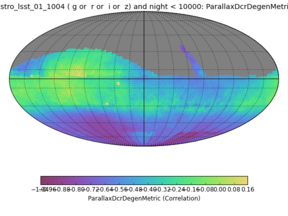
\includegraphics[width=2.0in]{./figs/milkyway/astromPanels/MW_Astrom_paDcrDegen_wfdPlane_10y_map.png}
  \end{center}

  \begin{center}
  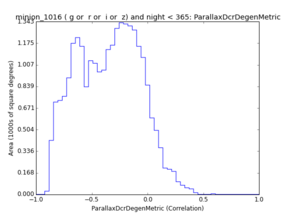
\includegraphics[width=2.0in]{./figs/milkyway/astromPanels/MW_Astrom_paDcrDegen_Baseline_01y_hst.png}
  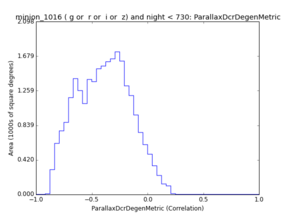
\includegraphics[width=2.0in]{./figs/milkyway/astromPanels/MW_Astrom_paDcrDegen_Baseline_02y_hst.png}
  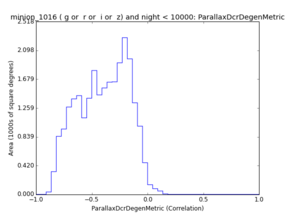
\includegraphics[width=2.0in]{./figs/milkyway/astromPanels/MW_Astrom_paDcrDegen_Baseline_10y_hst.png}
  \end{center}
  \begin{center}
  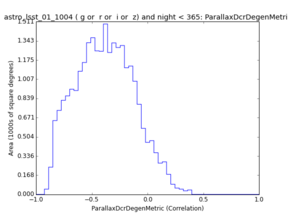
\includegraphics[width=2.0in]{./figs/milkyway/astromPanels/MW_Astrom_paDcrDegen_wfdPlane_01y_hst.png}
  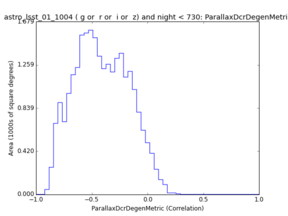
\includegraphics[width=2.0in]{./figs/milkyway/astromPanels/MW_Astrom_paDcrDegen_wfdPlane_02y_hst.png}
  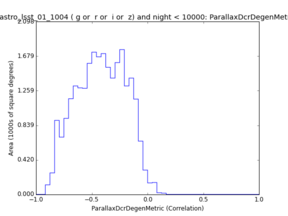
\includegraphics[width=2.0in]{./figs/milkyway/astromPanels/MW_Astrom_paDcrDegen_wfdPlane_10y_hst.png}
  \end{center}
  \caption{Correlation coefficient $\rho$~between parallax and Differential Chromatic Refraction (DCR) up to different epochs within the survey. {\it Top and Third row:} OpSim run \opsimdbref{db:baseCadence}. {\it Second and bottom row:} OpSim run \opsimdbref{db:NormalGalacticPlane} (wide-fast-deep extended to much of the inner Plane). Reading left-right, columns represent: {\it Left column:} all observations within the first 365 days of operation; {\it Middle column:} first two years; {\it right column:} the full 10-year survey. Spatial maps are clipped at 95\%, with histogram horizontal scale set to the range $-1.0 \le \rho \le +1.0$.}
  \label{fig_astrom_ByTime_PADegen}
\end{figure}



\begin{figure}[ht]
  \begin{center}
  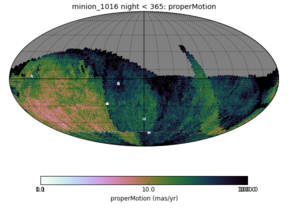
\includegraphics[width=2.0in]{./figs/milkyway/astromPanels/MW_Astrom_pmError_Baseline_01y_map.png}
  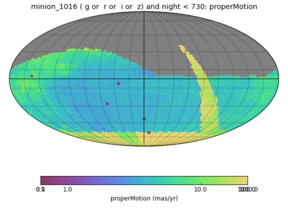
\includegraphics[width=2.0in]{./figs/milkyway/astromPanels/MW_Astrom_pmError_Baseline_02y_map.png}
  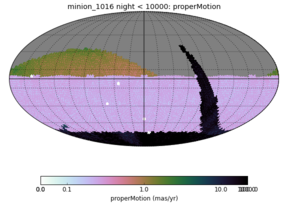
\includegraphics[width=2.0in]{./figs/milkyway/astromPanels/MW_Astrom_pmError_Baseline_10y_map.png}
  \end{center}
  \begin{center}
  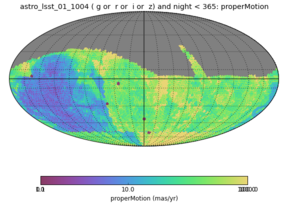
\includegraphics[width=2.0in]{./figs/milkyway/astromPanels/MW_Astrom_pmError_wfdPlane_01y_map.png}
  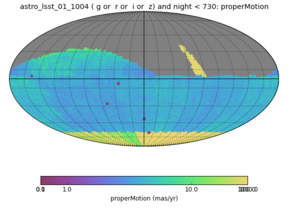
\includegraphics[width=2.0in]{./figs/milkyway/astromPanels/MW_Astrom_pmError_wfdPlane_02y_map.png}
  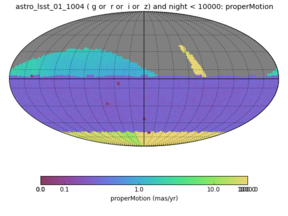
\includegraphics[width=2.0in]{./figs/milkyway/astromPanels/MW_Astrom_pmError_wfdPlane_10y_map.png}
  \end{center}

  \begin{center}
  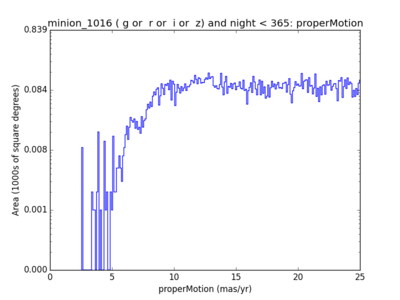
\includegraphics[width=2.0in]{./figs/milkyway/astromPanels/MW_Astrom_pmError_Baseline_01y_hst.png}
  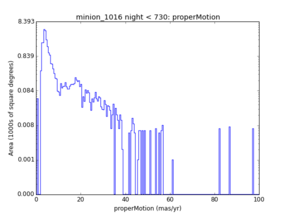
\includegraphics[width=2.0in]{./figs/milkyway/astromPanels/MW_Astrom_pmError_Baseline_02y_hst.png}
  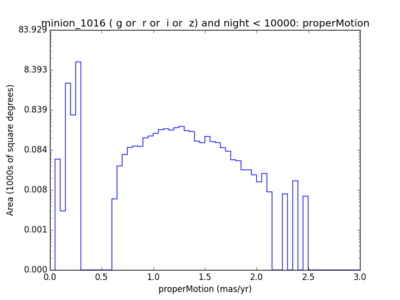
\includegraphics[width=2.0in]{./figs/milkyway/astromPanels/MW_Astrom_pmError_Baseline_10y_hst.png}
  \end{center}
  \begin{center}
  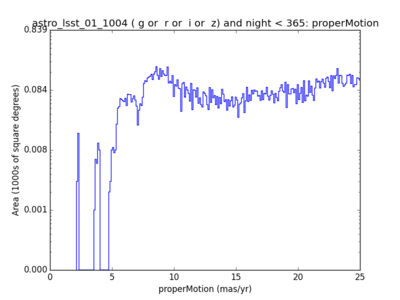
\includegraphics[width=2.0in]{./figs/milkyway/astromPanels/MW_Astrom_pmError_wfdPlane_01y_hst.png}
  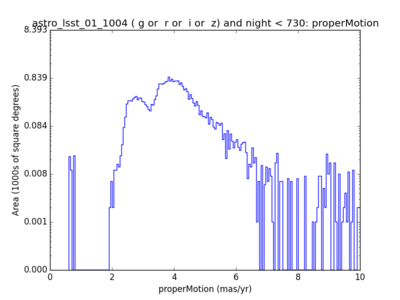
\includegraphics[width=2.0in]{./figs/milkyway/astromPanels/MW_Astrom_pmError_wfdPlane_02y_hst.png}
  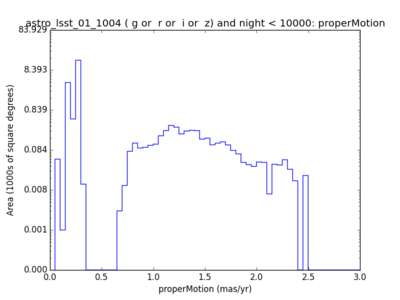
\includegraphics[width=2.0in]{./figs/milkyway/astromPanels/MW_Astrom_pmError_wfdPlane_10y_hst.png}
  \end{center}
  \caption{Proper motion error for a star at $r=21.0$, for different epochs within the survey. Crowding errors are ignored. {\it Top and Third row:} OpSim run \opsimdbref{db:baseCadence}.  {\it Second and bottom row:} OpSim run \opsimdbref{db:NormalGalacticPlane} (wide-fast-deep extended to much of the inner Plane). Reading left-right, columns represent: {\it Left column:} all observations within the first 365 days of operation; {\it Middle column:} first two years; {\it right column:} the full 10-year survey. Spatial maps are clipped at 95\% and a log-scale is used for the maps and histograms. Reading left-right, the horizontal upper limits on the histograms are (25, 10, 3.0) mas yr$^{-1}$, respectively. Note that the histograms do not include the full range of values reported in the maps.}
  \label{fig_astrom_ByTime_pmError}
\end{figure}


\begin{figure}[ht]
  \begin{center}
  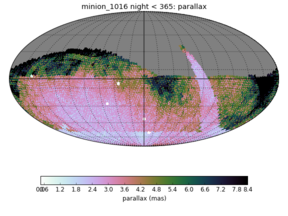
\includegraphics[width=2.0in]{./figs/milkyway/astromPanels/MW_Astrom_paError_Baseline_01y_map.png}
  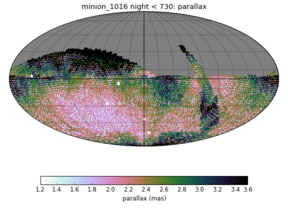
\includegraphics[width=2.0in]{./figs/milkyway/astromPanels/MW_Astrom_paError_Baseline_02y_map.png}
  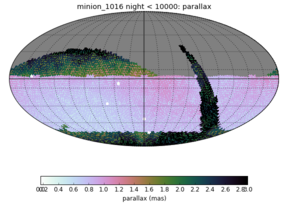
\includegraphics[width=2.0in]{./figs/milkyway/astromPanels/MW_Astrom_paError_Baseline_10y_map.png}
  \end{center}
  \begin{center}
  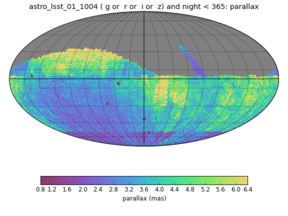
\includegraphics[width=2.0in]{./figs/milkyway/astromPanels/MW_Astrom_paError_wfdPlane_01y_map.png}
  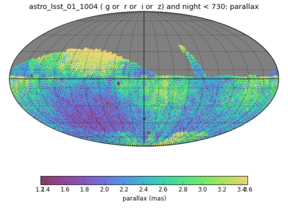
\includegraphics[width=2.0in]{./figs/milkyway/astromPanels/MW_Astrom_paError_wfdPlane_02y_map.png}
  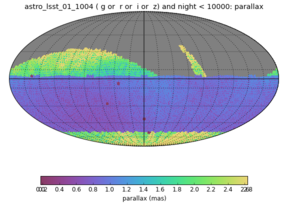
\includegraphics[width=2.0in]{./figs/milkyway/astromPanels/MW_Astrom_paError_wfdPlane_10y_map.png}
  \end{center}

  \begin{center}
  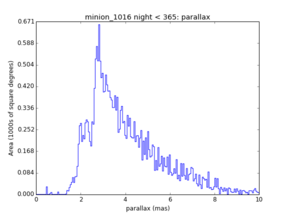
\includegraphics[width=2.0in]{./figs/milkyway/astromPanels/MW_Astrom_paError_Baseline_01y_hst.png}
  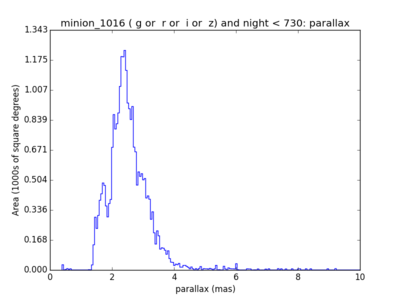
\includegraphics[width=2.0in]{./figs/milkyway/astromPanels/MW_Astrom_paError_Baseline_02y_hst.png}
  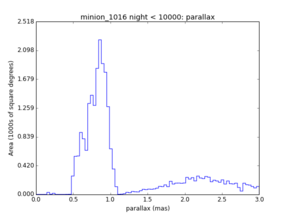
\includegraphics[width=2.0in]{./figs/milkyway/astromPanels/MW_Astrom_paError_Baseline_10y_hst.png}
  \end{center}
  \begin{center}
  \includegraphics[width=2.0in]{./figs/milkyway/astromPanels/MW_Astrom_paError_wfdPlane_01y_hst.png}
  \includegraphics[width=2.0in]{./figs/milkyway/astromPanels/MW_Astrom_paError_wfdPlane_02y_hst.png}
  \includegraphics[width=2.0in]{./figs/milkyway/astromPanels/MW_Astrom_paError_wfdPlane_10y_hst.png}
  \end{center}
  \caption{Parallax error for a star at $r=21.0$, for different epochs within the survey. Crowding errors are ignored. {\it Top and Third row:} OpSim run \opsimdbref{db:baseCadence}. {\it Second and bottom row:} OpSim run \opsimdbref{db:NormalGalacticPlane} (wide-fast-deep extended to much of the inner Plane). Reading left-right, columns represent: {\it Left column:} all observations within the first 365 days of operation; {\it Middle column:} first two years; {\it right column:} the full 10-year survey. Spatial maps are clipped at 95\%.  Reading left-right, the horizontal upper limits on the histograms are (10, 10, 2.0) mas, respectively.}
  \label{fig_astrom_ByTime_paError}
\end{figure}

%%% Now for the metrics by filter.
\begin{figure}[ht]
  \begin{center}
  \includegraphics[width=2.0in]{./figs/milkyway/astromPanels/MW_Astrom_paCovge_Baseline_u_map.png}
  \includegraphics[width=2.0in]{./figs/milkyway/astromPanels/MW_Astrom_paCovge_Baseline_y_map.png}
  \includegraphics[width=2.0in]{./figs/milkyway/astromPanels/MW_Astrom_paCovge_Baseline_10y_map.png}
  \end{center}
  \begin{center}
  \includegraphics[width=2.0in]{./figs/milkyway/astromPanels/MW_Astrom_paCovge_wfdPlane_u_map.png}
  \includegraphics[width=2.0in]{./figs/milkyway/astromPanels/MW_Astrom_paCovge_wfdPlane_y_map.png}
  \includegraphics[width=2.0in]{./figs/milkyway/astromPanels/MW_Astrom_paCovge_wfdPlane_10y_map.png}
  \end{center}

  \begin{center}
  \includegraphics[width=2.0in]{./figs/milkyway/astromPanels/MW_Astrom_paCovge_Baseline_u_hst.png}
  \includegraphics[width=2.0in]{./figs/milkyway/astromPanels/MW_Astrom_paCovge_Baseline_y_hst.png}
  \includegraphics[width=2.0in]{./figs/milkyway/astromPanels/MW_Astrom_paCovge_Baseline_10y_hst.png}
  \end{center}
  \begin{center}
  \includegraphics[width=2.0in]{./figs/milkyway/astromPanels/MW_Astrom_paCovge_wfdPlane_u_hst.png}
  \includegraphics[width=2.0in]{./figs/milkyway/astromPanels/MW_Astrom_paCovge_wfdPlane_y_hst.png}
  \includegraphics[width=2.0in]{./figs/milkyway/astromPanels/MW_Astrom_paCovge_wfdPlane_10y_hst.png}
  \end{center}
  \caption{Parallax coverage achieved for three extremes of object color, over the full 10-year survey. {\it Top and Third row:} OpSim run \opsimdbref{db:baseCadence}. {\it Second and bottom row:} OpSim run \opsimdbref{db:NormalGalacticPlane} (wide-fast-deep extended to much of the inner Plane). Reading left-right, columns represent: {\it Left column:} Objects detected only in the bluest filter; {\it Middle column:} objects detected only in the reddest filter; {\it Right column:} objects detected in all filters. Spatial maps are clipped at 95\%, with histogram horizontal limits (0.0 - 1.0).}
  \label{fig_astrom_ByFilter_PACoverage}
\end{figure}

\begin{figure}[ht]
  \begin{center}
  \includegraphics[width=2.0in]{./figs/milkyway/astromPanels/MW_Astrom_paDcrDegen_Baseline_u_map.png}
  \includegraphics[width=2.0in]{./figs/milkyway/astromPanels/MW_Astrom_paDcrDegen_Baseline_y_map.png}
  \includegraphics[width=2.0in]{./figs/milkyway/astromPanels/MW_Astrom_paDcrDegen_Baseline_10y_map.png}
  \end{center}
  \begin{center}
  \includegraphics[width=2.0in]{./figs/milkyway/astromPanels/MW_Astrom_paDcrDegen_wfdPlane_u_map.png}
  \includegraphics[width=2.0in]{./figs/milkyway/astromPanels/MW_Astrom_paDcrDegen_wfdPlane_y_map.png}
  \includegraphics[width=2.0in]{./figs/milkyway/astromPanels/MW_Astrom_paDcrDegen_wfdPlane_10y_map.png}
  \end{center}

  \begin{center}
  \includegraphics[width=2.0in]{./figs/milkyway/astromPanels/MW_Astrom_paDcrDegen_Baseline_u_hst.png}
  \includegraphics[width=2.0in]{./figs/milkyway/astromPanels/MW_Astrom_paDcrDegen_Baseline_y_hst.png}
  \includegraphics[width=2.0in]{./figs/milkyway/astromPanels/MW_Astrom_paDcrDegen_Baseline_10y_hst.png}
  \end{center}
  \begin{center}
  \includegraphics[width=2.0in]{./figs/milkyway/astromPanels/MW_Astrom_paDcrDegen_wfdPlane_u_hst.png}
  \includegraphics[width=2.0in]{./figs/milkyway/astromPanels/MW_Astrom_paDcrDegen_wfdPlane_y_hst.png}
  \includegraphics[width=2.0in]{./figs/milkyway/astromPanels/MW_Astrom_paDcrDegen_wfdPlane_10y_hst.png}
  \end{center}
  \caption{Correlation coefficient $\rho$~between parallax and Differential Chromatic Refraction (DCR), selecting filters for three extremes of object color, over the full 10-year survey. {\it Top and Third row:} OpSim run \opsimdbref{db:baseCadence}. {\it Second and bottom row:} OpSim run \opsimdbref{db:NormalGalacticPlane} (wide-fast-deep extended to much of the inner Plane). Reading left-right, columns represent: {\it Left column:} Objects detected only in the bluest filter; {\it Middle column:} objects detected only in the reddest filter; {\it Right column:} objects detected in all filters. Spatial maps are clipped at 95\%, with histogram horizontal scale set to the range $-1.0 \le \rho \le +1.0$.}
  \label{fig_astrom_ByFilter_PADegen}
\end{figure}

\begin{figure}[ht]
  \begin{center}
  \includegraphics[width=2.0in]{./figs/milkyway/astromPanels/MW_Astrom_pmError_Baseline_u_map.png}
  \includegraphics[width=2.0in]{./figs/milkyway/astromPanels/MW_Astrom_pmError_Baseline_y_map.png}
  \includegraphics[width=2.0in]{./figs/milkyway/astromPanels/MW_Astrom_pmError_Baseline_10y_map.png}
  \end{center}
  \begin{center}
  \includegraphics[width=2.0in]{./figs/milkyway/astromPanels/MW_Astrom_pmError_wfdPlane_u_map.png}
  \includegraphics[width=2.0in]{./figs/milkyway/astromPanels/MW_Astrom_pmError_wfdPlane_y_map.png}
  \includegraphics[width=2.0in]{./figs/milkyway/astromPanels/MW_Astrom_pmError_wfdPlane_10y_map.png}
  \end{center}

  \begin{center}
  \includegraphics[width=2.0in]{./figs/milkyway/astromPanels/MW_Astrom_pmError_Baseline_u_hst.png}
  \includegraphics[width=2.0in]{./figs/milkyway/astromPanels/MW_Astrom_pmError_Baseline_y_hst.png}
  \includegraphics[width=2.0in]{./figs/milkyway/astromPanels/MW_Astrom_pmError_Baseline_10y_hst.png}
  \end{center}
  \begin{center}
  \includegraphics[width=2.0in]{./figs/milkyway/astromPanels/MW_Astrom_pmError_wfdPlane_u_hst.png}
  \includegraphics[width=2.0in]{./figs/milkyway/astromPanels/MW_Astrom_pmError_wfdPlane_y_hst.png}
  \includegraphics[width=2.0in]{./figs/milkyway/astromPanels/MW_Astrom_pmError_wfdPlane_10y_hst.png}
  \end{center}
  \caption{Proper motion error for a star at apparent magnitude $m=21.0$, for three extremes of object color and assessed over the full survey. Crowding errors are ignored. {\it Top and Third row:} OpSim run \opsimdbref{db:baseCadence}. {\it Second and bottom row:} OpSim run \opsimdbref{db:NormalGalacticPlane} (wide-fast-deep extended to much of the inner Plane). Reading left-right, columns represent: {\it Left column:} Objects detected only in the bluest filter; the fiducial object has apparent magnitude $u=21.0$; {\it Middle column:} objects detected only in the reddest filter (so $y = 21.0$); {\it Right column:} objects detected in all filters (using $r=21.0$~and a ``flat'' spectrum within sims\_maf). Spatial maps are clipped at 95\% and a log-scale is used for both the spatial maps and histograms. Reading left-right, the horizontal upper limits on the histograms are (4.0, 4.0, 3.0) mas yr$^{-1}$, respectively. Note that the histograms do not include the full range of values reported in the maps.}
  \label{fig_astrom_ByFilter_pmError}
\end{figure}

\begin{figure}[ht]
  \begin{center}
  \includegraphics[width=2.0in]{./figs/milkyway/astromPanels/MW_Astrom_paError_Baseline_u_map.png}
  \includegraphics[width=2.0in]{./figs/milkyway/astromPanels/MW_Astrom_paError_Baseline_y_map.png}
  \includegraphics[width=2.0in]{./figs/milkyway/astromPanels/MW_Astrom_paError_Baseline_10y_map.png}
  \end{center}
  \begin{center}
  \includegraphics[width=2.0in]{./figs/milkyway/astromPanels/MW_Astrom_paError_wfdPlane_u_map.png}
  \includegraphics[width=2.0in]{./figs/milkyway/astromPanels/MW_Astrom_paError_wfdPlane_y_map.png}
  \includegraphics[width=2.0in]{./figs/milkyway/astromPanels/MW_Astrom_paError_wfdPlane_10y_map.png}
  \end{center}

  \begin{center}
  \includegraphics[width=2.0in]{./figs/milkyway/astromPanels/MW_Astrom_paError_Baseline_u_hst.png}
  \includegraphics[width=2.0in]{./figs/milkyway/astromPanels/MW_Astrom_paError_Baseline_y_hst.png}
  \includegraphics[width=2.0in]{./figs/milkyway/astromPanels/MW_Astrom_paError_Baseline_10y_hst.png}
  \end{center}
  \begin{center}
  \includegraphics[width=2.0in]{./figs/milkyway/astromPanels/MW_Astrom_paError_wfdPlane_u_hst.png}
  \includegraphics[width=2.0in]{./figs/milkyway/astromPanels/MW_Astrom_paError_wfdPlane_y_hst.png}
  \includegraphics[width=2.0in]{./figs/milkyway/astromPanels/MW_Astrom_paError_wfdPlane_10y_hst.png}
  \end{center}
  \caption{Parallax error for a star at apparent magnitude $m=21.0$, for three extremes of object color and assessed over the full survey. Crowding errors are ignored. {\it Top and Third row:} OpSim run \opsimdbref{db:baseCadence}. {\it Second and bottom row:} OpSim run \opsimdbref{db:NormalGalacticPlane} (wide-fast-deep extended to much of the inner Plane). Reading left-right, columns represent: {\it Left column:} Objects detected only in the bluest filter; the fiducial object has apparent magnitude $u=21.0$; {\it Middle column:} objects detected only in the reddest filter (so $y = 21.0$); {\it Right column:} objects detected in all filters (using $r=21.0$~and a ``flat'' spectrum within sims\_maf). Spatial maps are clipped at 95\%. Reading left-right, the horizontal upper limits on the histograms are (10, 10, 2.0) mas, respectively. Note that the histograms do not include the full range of values reported in the maps.}
  \label{fig_astrom_ByFilter_paError}
\end{figure}

\subsubsection{Figures of Merit depending on the Metrics}

Building on the first-order metrics above, this subsection communicates scientific figures of merit for the cases identified in \autoref{sec:\secname:MW_Astrometry_measurements} above.

Table \ref{tab_SummaryMWAstrometry} summarizes the Figures of Merit
(FoMs) for Astrometry science cases. At the time of writing, FoMs have
been implemented to summarize the random uncertainty in proper motion
and parallax, for two regions experiencing extreme values of these
quantities: the inner Plane (conservatively defined in this section as
$|b| \lesssim 7^o$~and $|l| \lesssim 80^o$), and the main survey
(excluding the inner plane and the Southern Polar region, taken
here as $\delta_{2000.0} < -60.0^o$). Figure
\ref{fig_astrom_RegionSelKey} illustrates these selection-regions on
the sky. These form FoM 1.1-1.4, and have to-date been run for the
OpSim runs \opsimdbref{db:baseCadence} (Baseline cadence),
\opsimdbref{db:opstwoPS} (similar to PanSTARRS-1), and the
recently-completed \opsimdbref{db:NormalGalacticPlane} (which applies
Wide-Fast-Deep cadence to much of the inner Galactic Plane). From the point of
view of parallax and proper motion, the latter two strategies do not
negatively impact the non-plane regions, but they {\it substantially}
improve the sampling for proper motions and parallax (again,
neglecting the effects of spatial crowding).

FoM 1.5 in Table \ref{tab_SummaryMWAstrometry} reports the total number of fields with Parallax/Hour-angle correlation $|\rho| < 0.7$.

At the time of writing, FoMs 2-5 in Table
\ref{tab_SummaryMWAstrometry} are still at the specification stage,
and are described in Section
\ref{sec:\secname:MW_Astrometry_furtherwork}.

%%%% Figures used as ``key'' for the astrometry FoMs:

\begin{figure}[h]
  \begin{center}
    \includegraphics[width=2.0in]{./figs/milkyway/astromPanels/MW_Astrom_FoM_properMotion_minion_1016_all_skymap.png}
  \includegraphics[width=2.0in]{./figs/milkyway/astromPanels/MW_Astrom_FoM_properMotion_minion_1016_plane_skymap.png}
  \includegraphics[width=2.0in]{./figs/milkyway/astromPanels/MW_Astrom_FoM_properMotion_minion_1016_nonPlane_skymap.png}
    \end{center}
  \caption{Selection regions for the Astrometry Figures of Merit (FoMs) 1.1-1.4. Figures of Merit 1.1 and 1.3 refer to the ``main survey'' region shown in the middle panel (which for the FoM also avoids the region of the South Galactic Pole). The right panel shows the inner Plane region to which FoMs 1.2 \& 1.4 refer. The left-hand panel shows the entire survey region for reference. This example shows run \opsimdbref{db:baseCadence}. See Table \ref{tab_SummaryMWAstrometry} and Section \ref{sec:\secname:MW_Astrometry_metrics}.}
  \label{fig_astrom_RegionSelKey}
\end{figure}

\subsection{Topics that will need to be addressed}
\label{sec:\secname:MW_Astrometry_furtherwork}

Here we present suggestions for further work, first on figures of
merit for the science cases, and then on additional Metrics for LSST's
astrometric performance.

\subsubsection{Further work on science Figures of Merit}
%\medskip

At the time of writing, the Figures of Merit for both the highlighted
Science cases need to be implemented and applied to OpSim output,
preferably in a format that can be summarized in a single Table in
this section. These figures of merit are discussed above in Section
\ref{sec:\secname:MW_Astrometry_metrics} (particularly for the Halo
Streams science project). Figures of merit for the two science cases
might be:
\begin{itemize}
  \item[1.] Number of streams that LSST can discover via their proper motions;
\item[2.] Uncertainty and bias in the thin and thick disk differential age measurement when using white dwarfs from each population as tracers.
\end{itemize}

Given the diversity of science cases that use local Solar Neighborhood
populations as tracers, it may be advantageous to subdivide the Solar
Neighborhood projects into further figures of merit. Two further example
figures of merit might then be:
\begin{itemize}
  \item[3.] Uncertainty and bias in the Brown Dwarf mass function using Solar Neighborhood tracers;
   \item[4.] Uncertainty and bias in the thickness in the main sequence of M-dwarfs within 25pc from the Sun, once variability has been characterized and removed.
\end{itemize}

%%%% SUMMARY TABLE FOR THIS SECTION

\begin{table}
  \begin{tabular}{l|p{4.8cm}|p{1.1cm}|p{1.1cm}|p{1.1cm}|c|p{3.5cm}}
    FoM & Brief description & {\rotatebox{90}{\opsimdbref{db:baseCadence} }} & {\rotatebox{90}{\opsimdbref{db:opstwoPS} }} & {\rotatebox{90}{\opsimdbref{db:NormalGalacticPlane}   }} &  {\rotatebox{90}{future run 2}} & Notes \\
    \hline
    1.1 & \footnotesize{Median parallax error at $r=21$ (main survey)}      & 0.69  & 0.72 & 0.69 & - &
%\footnotesize{Summarize the presentation in Figures \ref{fig_astrom_ByTime_PACoverage}-\ref{fig_astrom_ByFilter_paError} }
\footnotesize{See region definitions in Figure \ref{fig_astrom_RegionSelKey}.}
\\
    1.2. & \footnotesize{Median parallax error at $r=21$ (plane)}   & 2.68 & {\bf 0.91} & {\bf 0.89} & - &
\footnotesize{Smaller values are better.}\\
    1.3. & \footnotesize{Median proper motion error at $r=21$ (main survey)}  & 0.19 & 0.19 & 0.19 & - &
%\footnotesize{Take median of Figure \ref{fig_astrom_ByTime_pmError} over the ``plane'' region.}
\\
    1.4. & \footnotesize{Median proper motion error at $r=21$ (plane)} & 16.7
%$^\dagger$
& {\bf 0.26} & {\bf 0.25} & - &
%\footnotesize{$^\dagger$no, this is not a typo.}
\\
1.5. & \footnotesize{Fields with Parallax-DCR correlation coefficient $\rho \ge 0.7$~/ total fields} & \footnotesize{ \bf{3486} / \bf {31116} } & \footnotesize{3586 / 30107} & \footnotesize{3690 / 31116} & - & \footnotesize{Smaller is better. Value reported after full 10 years of survey for $griz$~detections.}  \\
    \hline
    2.1. & \footnotesize{Number of streams LSST can discover via proper motions} & - & - & - & - &  - \\
    3.1. & \footnotesize{Uncertainty and bias in thin- and thick-disk differential age measurement via white dwarfs} & - & - & - & - &  - \\
    4.1. & \footnotesize{Uncertainty and bias in brown dwarf mass function from the Solar Neighborhood}  & - & - & - & - & \footnotesize{Using astrometry metrics for objects detected only in the reddest filter(s)} \\
    4.2. & \footnotesize{Uncertainty and bias in white dwarf mass function from the Solar Neighborhood}  & - & - & - & - & \footnotesize{Using astrometry metrics for objects detected only in the bluest filter(s)} \\
    5.1. & \footnotesize{Uncertainty and bias in Solar Neighborhood M-dwarf thickness on the MS}  & - & - & - & - &  - \\
\end{tabular}
\caption{Summary of Figures of Merit for the Milky Way Astrometry science cases. The best value of each FoM is indicated in bold. Runs \opsimdbref{db:baseCadence} and \opsimdbref{db:opstwoPS} refer to the Baseline and PanSTARRS-like strategies, respectively. Column \opsimdbref{db:NormalGalacticPlane} refers to a recently-completed OpSim run that includes the Plane in Wide-Fast-Deep observations. See \autoref{sec:MW_Astrometry}.}
\label{tab_SummaryMWAstrometry}
\end{table}


%%%% SUMMARY TABLE FINISHES HERE


\subsubsection{Further work on Astrometry Metrics}

The MAF metrics presented in Sections \ref{sec:\secname:MW_Astrometry_OpSim} and \ref{sec:\secname:MW_Astrometry_metrics} are only part of the
study of LSST's predicted astrometric performance.  Detailed simulations
and studies need to be done in many other areas as part of the
prediction and verification of LSST's astrometric performance.  Among
the most important are the following.
\begin{itemize}
\item How well do galaxies perform as astrometric reference objects? Are certain shapes or colors better than others? What is the
surface density of ``good" astrometric reference galaxies as a function of filter?
\item How well can we identify optically point-like QSOs that will be useful in matching the optical reference frame to the ICRS?
%\item Given the LSST exposure time, site, and physical characteristics, how can we mitigate the limitations on astrometric accuracy imposed by the seeing and local atmospheric turbulence?
\item How does the astrometric performance depend on stellar density? If there are fields in which photometry is only possible via difference imaging, what are the limitations
on astrometry in these fields?
%\item What tools do we need to compare the general and specific agreement between the {\it Gaia} results and the LSST results?
\item Does the ``brighter-wider" effect in the deep-depletion CCDs introduce a magnitude term into the centroid positions?
\end{itemize}

% ====================================================================

\subsection{Conclusions}

Here we answer the ten questions posed in
\autoref{sec:intro:evaluation:caseConclusions}:

\begin{description}

\item[Q1:] {\it Does the science case place any constraints on the
tradeoff between the sky coverage and coadded depth? For example, should
the sky coverage be maximized (to $\sim$30,000 deg$^2$, as e.g., in
Pan-STARRS) or the number of detected galaxies (the current baseline but
with 18,000 deg$^2$)?}

\new{ \item[A1:] We do expect tradeoffs between depth and sky
  coverage, but we do not yet have the FoM evaluations to set
  quantitative constraints. For example, we expect some combination of
  depth and survey volume would optimize the completeness to objects
  among the populations in the Solar Neighborhood. More generally,
  perhaps, in fields away from the galactic mid-plane, the
  lengthscales over which the proper motion zeropoints can be
  accurately constrained will depend on the spatial density of
  well-measured background galaxies (finer lengthscale corresponding
  to greater co-added depth). The depth must therefore be sufficient
  to sample enough of these galaxies to constrain variations of
  astrometric zeropoint on lengthscales at least as fine as those
  imposed by the LSST system itself (or the atmosphere, whichever is
  finer). We anticipate that this tradeoff can be informed by
  simulation under a set of assumptions for these variations.}

\item[Q2:] {\it Does the science case place any constraints on the
tradeoff between uniformity of sampling and frequency of  sampling? For
example, a rolling cadence can provide enhanced sample rates over a part
of the survey or the entire survey for a designated time at the cost of
reduced sample rate the rest of the time (while maintaining the nominal
total visit counts).}

\new{ \item[A2:] Yes, although for astrometry the language of these
  constraints is slightly different. The parallactic ellipse must be
  sufficiently covered, the correlation between hour angle and
  parallax factor must be minimized, and the visits must be
  sufficiently distributed (both within a year and over the ten-year
  time baseline) to produce the best precision in both proper motion and parallax. See Section \ref{sec:MW_Astrometry:MW_Astrometry_metrics}}.

\item[Q3:] {\it Does the science case place any constraints on the
tradeoff between the single-visit depth and the number of visits
(especially in the $u$-band where longer exposures would minimize the
impact of the readout noise)?}

\new{ \item[A3:] More visits at the standard exposure time are
  generally preferred to a few visits with longer exposures, in order
  to achieve as broad a temporal coverage as possible (see Section
  \ref{sec:MW_Astrometry:MW_Astrometry_metrics}). The $u$-band itself
  is likely to be of limited use for astrometry (except possibly for
  extremely blue objects with little signal in any of the other
  filters) due to differential chromatic refraction (DCR), however of
  course $u$-band will still be useful for photometric constraints.}

\item[Q4:] {\it Does the science case place any constraints on the
Galactic plane coverage (spatial coverage, temporal sampling, visits per
band)?}

\new{ \item[A4:] Not for the example of detecting Galactic Halo
  streams via proper motions (Section
  \ref{sec:MW_Astrometry:MW_Astrometry_measurements}). For the Solar
  Neighborhood populations, avoiding the inner Galactic mid-plane
  would obviously reduce the completeness of the census of nearby
  objects with parallax determinations due to the reduction in total
  area surveyed. However, this reduction may be incremental rather
  than serious. The impact of an inner-plane zone of avoidance on the
  recovery of the parameters describing these constituent populations
  has not yet been evaluated. Of course, this all changes for
  astrometry of objects of interest that lie in the inner plane (see
  also Section \ref{sec:MW_Disk}), where (for example) the reduced
  proper motion will be a useful diagnostic. At present, however, the
  performance of the LSST software stack towards crowded fields is
  as-yet unknown. As this performance becomes better understood, it
  will be possible to quantitatively compare strategies for astrometry
  towards the inner plane.}

\item[Q5:] {\it Does the science case place any constraints on the
fraction of observing time allocated to each band?}

\new{ \item[A5:] Yes, but indirectly through the requirement to
  measure all the populations of interest in the Solar
  Neighborhood. Making the assumption that this science case requires
  parallax measurements for extremely blue objects as well as
  extremely red objects, which might each be measurable only in a
  single very red or blue filter, would suggest at a minimum that the
  coverage considerations of Section
  \ref{sec:MW_Astrometry:MW_Astrometry_metrics} be applied to
  observations in $u$~and $Y$ filters separately, as well as at least
  one mid-range filter. However the quantitative impact on population
  recovery from various filter-distributions has yet to be assessed at
  this date. Further work is needed to determine if the increased
  sensitivity of $u$-band astrometry to DCR relative to $g$-band would
  prevent its use for astrometry.}

\item[Q6:] {\it Does the science case place any constraints on the
cadence for deep drilling fields?}

\new{ \item[A6:] If precision astrometry is desired for the deep drilling fields, then the considerations of Section \ref{sec:MW_Astrometry:MW_Astrometry_metrics} apply to those fields as well.}

\item[Q7:] {\it Assuming two visits per night, would the science case
benefit if they are obtained in the same band or not?}

\new{ \item[A7:] While detailed investigation is still pending, we
  expect that using different filters within the same night would be
  preferred to allow better constraint of DCR effects. Doing different
  filters on the same night might reduce the number of free parameters
  (like seeing and parallax factor) and give more pairs for direct
  filter-A vs. filter-B astrometry.}

\item[Q8:] {\it Will the case science benefit from a special cadence
prescription during commissioning or early in the survey, such as:
acquiring a full 10-year count of visits for a small area (either in all
the bands or in a  selected set); a greatly enhanced cadence for a small
area?}

\new{ \item[A8:] It is vital for astrometry that at least a few fields
  be observed with both sufficient parallax factor coverage and
  sufficient number of visits, early in the survey, to demonstrate
  parallax precision specified in the Science Requirements
  Document. In these fields, sufficient exposures must be reserved for
  the entire 10-year survey baseline so that proper motion precision
  is not too badly compromised in these fields. This combination of
  factors may require dedicated commissioning observations of these
  fields in addition to the 10-year survey operations. In addition,
  however, at least a few fields must be observed at a variety of
  values of single-visit achieved depth, and FWHM, in order to
  constrain the degree to which FWHM will actually predict the
  achieved astrometric precision (see also the answer to Q10
  below). This second set of requirements may also be best served by
  dedicated commissioning observations.}

\item[Q9:] {\it Does the science case place any constraints on the
sampling of observing conditions (e.g., seeing, dark sky, airmass),
possibly as a function of band, etc.?}

\new{ \item[A9:] The observations need to be planned in such a way
  that the correlation between parallax and hour-angle is minimized,
  to avoid deneracies between the motion due to atmospheric refraction and the motion that is sought due to parallax. See
  Section \ref{sec:MW_Astrometry:MW_Astrometry_metrics}.}

\item[Q10:] {\it Does the case have science drivers that would require
real-time exposure time optimization to obtain nearly constant
single-visit limiting depth?}

\new{ \item[A10:] While optimization on an exposure-to-exposure basis
  is perhaps unlikely, {\it selection} between observations in
  response to conditions (on a timescale of perhaps 10 minutes) will
  be crucial to maximize achieved astrometric precision. The rules by
  which this selection would proceed, still need to be charted. For
  example, while maintaining limiting depth might suggest shorter
  exposure times when the FWHM is narrow, this may not translate to
  improved astrometric error across an LSST chip, because the
  lengthscales of the turbulence driving the FWHM is not the same as
  that of the turbulence driving astrometric error across an LSST chip.}

\end{description}

\navigationbar

% --------------------------------------------------------------------

%% ====================================================================
%+
% SECTION:
%    section-name.tex  % eg lenstimedelays.tex
%
% CHAPTER:
%    chapter.tex  % eg cosmology.tex
%
% ELEVATOR PITCH:
%    Explain in a few sentences what the relevant discovery or
%    measurement is going to be discussed, and what will be important
%    about it. This is for the browsing reader to get a quick feel
%    for what this section is about.
%
% COMMENTS:
%
%
% BUGS:
%
%
% AUTHORS:
%    Phil Marshall (@drphilmarshall)  - put your name and GitHub username here!
%-
% ====================================================================

\section{Mapping the Milky Way Bulge}
\def\secname{MW_Bulge}\label{sec:\secname} % For example, replace "keyword" with "lenstimedelays"

\noindent{\it Will Clarkson, ...}  % (Writing team)

% This individual section will need to describe the particular
% discoveries and measurements that are being targeted in this section's
% science case. It will be helpful to think of a ``science case" as a
% ``science project" that the authors {\it actually plan to do}. Then,
% the sections can follow the tried and tested format of an observing
% proposal: a brief description of the investigation, with references,
% followed by a technical feasibility piece. This latter part will need
% to be quantified using the MAF framework, via a set of metrics that
% need to be computed for any given observing strategy to quantify its
% impact on the described science case. Ideally, these metrics would be
% combined in a well-motivated figure of merit. The section can conclude
% with a discussion of any risks that have been identified, and how
% these could be mitigated.

A short preamble goes here. What's the context for this science
project? Where does it fit in the big picture?

% --------------------------------------------------------------------

\subsection{Target measurements and discoveries}
\label{sec:\secname:MW_Bulge_targets}

Describe the discoveries and measurements you want to make.

Now, describe their response to the observing strategy. Qualitatively,
how will the science project be affected by the observing schedule and
conditions? In broad terms, how would we expect the observing strategy
to be optimized for this science?


% --------------------------------------------------------------------

\subsection{Metrics}
\label{sec:\secname:MW_Bulge_metrics}

Quantifying the response via MAF metrics: definition of the metrics,
and any derived overall figure of merit.


% --------------------------------------------------------------------

\subsection{OpSim Analysis}
\label{sec:\secname:MW_Bulge_analysis}

OpSim analysis: how good would the default observing strategy be, at
the time of writing for this science project?


% --------------------------------------------------------------------

\subsection{Discussion}
\label{sec:\secname:MW_Bulge_discussion}

Discussion: what risks have been identified? What suggestions could be
made to improve this science project's figure of merit, and mitigate
the identified risks?


% ====================================================================

\navigationbar

%% ====================================================================
%+
% SECTION:
%    section-name.tex  % eg lenstimedelays.tex
%
% CHAPTER:
%    chapter.tex  % eg cosmology.tex
%
% ELEVATOR PITCH:
%    Explain in a few sentences what the relevant discovery or
%    measurement is going to be discussed, and what will be important
%    about it. This is for the browsing reader to get a quick feel
%    for what this section is about.
%
% COMMENTS:
%
%
% BUGS:
%
%
% AUTHORS:
%    Phil Marshall (@drphilmarshall)  - put your name and GitHub username here!
%-
% ====================================================================

\section{Mapping the Local Volume with Resolved Stars}
\def\secname{MW_LocalVolume}\label{sec:\secname} % For example, replace "keyword" with "lenstimedelays"

\noindent{\it ???, ...}  % (Writing team)

% This individual section will need to describe the particular
% discoveries and measurements that are being targeted in this section's
% science case. It will be helpful to think of a ``science case" as a
% ``science project" that the authors {\it actually plan to do}. Then,
% the sections can follow the tried and tested format of an observing
% proposal: a brief description of the investigation, with references,
% followed by a technical feasibility piece. This latter part will need
% to be quantified using the MAF framework, via a set of metrics that
% need to be computed for any given observing strategy to quantify its
% impact on the described science case. Ideally, these metrics would be
% combined in a well-motivated figure of merit. The section can conclude
% with a discussion of any risks that have been identified, and how
% these could be mitigated.

A short preamble goes here. What's the context for this science
project? Where does it fit in the big picture?

% --------------------------------------------------------------------

\subsection{Target measurements and discoveries}
\label{sec:\secname:MW_LocalVolume_targets}

Describe the discoveries and measurements you want to make.

Now, describe their response to the observing strategy. Qualitatively,
how will the science project be affected by the observing schedule and
conditions? In broad terms, how would we expect the observing strategy
to be optimized for this science?


% --------------------------------------------------------------------

\subsection{Metrics}
\label{sec:\secname:MW_LocalVolume_metrics}

Quantifying the response via MAF metrics: definition of the metrics,
and any derived overall figure of merit.


% --------------------------------------------------------------------

\subsection{OpSim Analysis}
\label{sec:\secname:MW_LocalVolume_analysis}

OpSim analysis: how good would the default observing strategy be, at
the time of writing for this science project?


% --------------------------------------------------------------------

\subsection{Discussion}
\label{sec:\secname:MW_LocalVolume_discussion}

Discussion: what risks have been identified? What suggestions could be
made to improve this science project's figure of merit, and mitigate
the identified risks?


% ====================================================================

\navigationbar

% ====================================================================
%+
% SECTION:
%    section-name.tex  % eg lenstimedelays.tex
%
% CHAPTER:
%    chapter.tex  % eg cosmology.tex
%
% ELEVATOR PITCH:
%    Explain in a few sentences what the relevant discovery or
%    measurement is going to be discussed, and what will be important
%    about it. This is for the browsing reader to get a quick feel
%    for what this section is about.
%
% COMMENTS:
%
%
% BUGS:
%
%
% AUTHORS:
%    Phil Marshall (@drphilmarshall)  - put your name and GitHub username here!
%-
% ====================================================================

\section{Ongoing Developments}
\def\secname{MW_Future}\label{sec:\secname} % For example, replace "keyword" with "lenstimedelays"

\noindent{\it Will Clarkson, Kathy Vivas ...}  % (Writing team)

% This individual section will need to describe the particular
% discoveries and measurements that are being targeted in this section's
% science case. It will be helpful to think of a ``science case" as a
% ``science project" that the authors {\it actually plan to do}. Then,
% the sections can follow the tried and tested format of an observing
% proposal: a brief description of the investigation, with references,
% followed by a technical feasibility piece. This latter part will need
% to be quantified using the MAF framework, via a set of metrics that
% need to be computed for any given observing strategy to quantify its
% impact on the described science case. Ideally, these metrics would be
% combined in a well-motivated figure of merit. The section can conclude
% with a discussion of any risks that have been identified, and how
% these could be mitigated.

\new{This Section contains extremely brief initial notes for important
  science cases that (as of the current writing in mid-April 2016) are
  in an earlier stage of development than the cases in the previous
  sections. However we do not want these invesigations to drop off the
  radar.}

%A short preamble goes here. What's the context for this science
%project? Where does it fit in the big picture?

%% --------------------------------------------------------------------

\subsection{Target measurements and discoveries}
\label{sec:\secname:MW_Future_targets}

%Describe the discoveries and measurements you want to make.

\begin{itemize}
  \item {\it Formation history of the Bulge and present-day balance of populations:} Sensitivity to metallicity and age distribution of Bulge objects near the Main Sequence Turn-off;
    \item {\it Migration and heating in the Milky Way disk:} Error and bias in the determination of components in the (velocity dispersion vs metallicity) diagram, for disk populations along various lines of sight (e.g. Loebman et al. 2016 ApJ 818 L6);
    \item Fraction of Local-Volume objects discovered as a function of survey strategy
\end{itemize}

%Now, describe their response to the observing strategy. Qualitatively,
%how will the science project be affected by the observing schedule and
%conditions? In broad terms, how would we expect the observing strategy
%to be optimized for this science?


% --------------------------------------------------------------------

%\subsection{Metrics}
%\label{sec:\secname:MW_Bulge_metrics}

%Quantifying the response via MAF metrics: definition of the metrics,
%and any derived overall figure of merit.


% --------------------------------------------------------------------

%\subsection{OpSim Analysis}
%\label{sec:\secname:MW_Bulge_analysis}

%OpSim analysis: how good would the default observing strategy be, at
%the time of writing for this science project?


% --------------------------------------------------------------------

%\subsection{Discussion}
%\label{sec:\secname:MW_Bulge_discussion}

%Discussion: what risks have been identified? What suggestions could be
%made to improve this science project's figure of merit, and mitigate
%the identified risks?


% ====================================================================

\navigationbar

